\chapter{Descrizione del progetto}


L'applicazione desktop, sviluppata in Java, che è stata rivisitata in questo elaborato è \textit{BarattoManager}. Questa è stata progettata per il corso di Ingegneria del Software con l'obiettivo di familiarizzare con i casi d'uso e il risultato grafico non risulta essere avanzato.
In questo elaborato si è portato il progetto a un livello superiore, adeguandolo ai criteri di usabilità affrontati nel corso di Interazione Persona-Calcolatore.

L'applicazione permette agli utenti di scambiare articoli tra loro attraverso il baratto, quindi intende instaurare un sistema di scambio diretto di beni tra persone senza l'uso di denaro.
Gli articoli sono organizzati in una gerarchia di categorie, sottocategorie e campi descrittivi, e gli scambi si concludono con un appuntamento in uno dei luoghi e orari di incontro previsti dal sistema.

\section{La Schermata di Benvenuto (Login e Registrazione)}
All'avvio dell'applicazione, chiunque si trova davanti a una schermata di benvenuto. Da qui è possibile:
\begin{itemize}
    \item \textbf{Registrarsi}: un nuovo utente può creare il proprio account inserendo nome utente e password.
    \item  \textbf{Accedere}: inserendo le proprie credenziali.
\end{itemize}

\begin{figure}[H]
    \centering
    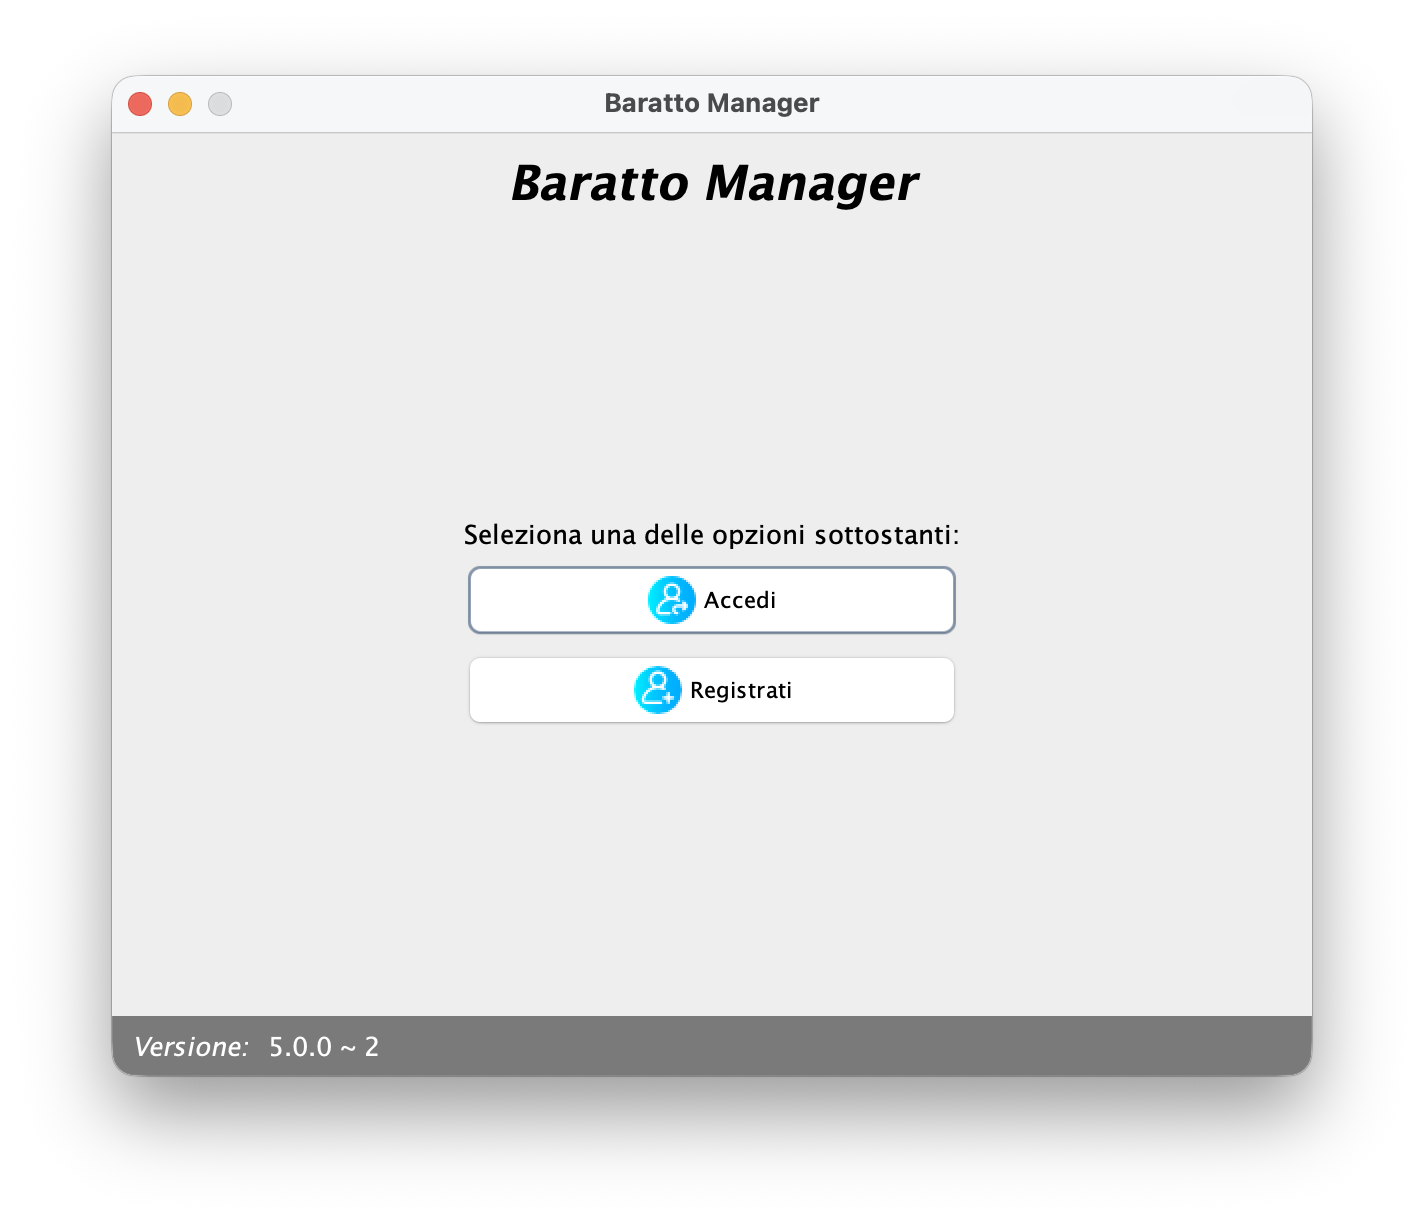
\includegraphics[width=0.5\linewidth]{figures/ss_UI_vecchia/HomePage.png}
    \caption{HomePage}
\end{figure}

Durante il primo accesso per un utente il sistema mostrerà immediatamente un avviso bloccante, obbligandolo a scegliere una nuova password personale prima di poter entrare.

\begin{figure}[H]
    \centering
    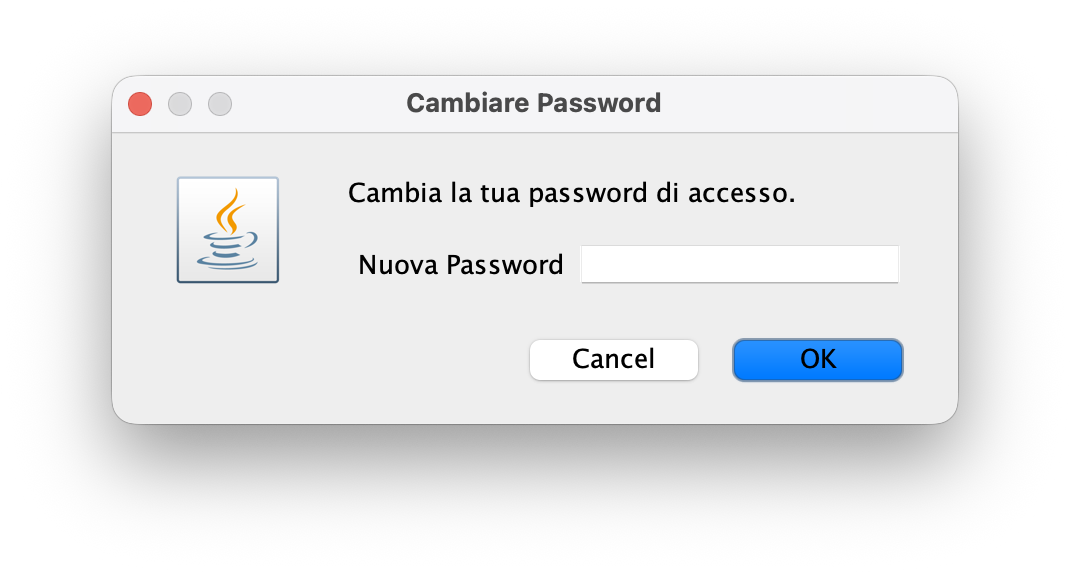
\includegraphics[width=0.5\linewidth]{figures/ss_UI_vecchia/Utente/CambioPassword.png}
    \caption{Avviso bloccante}
\end{figure}

Una volta effettuato l'accesso, il sistema riconosce automaticamente se chi è entrato è un \textbf{Configuratore} (l'amministratore del sistema) o un normale \textbf{Fruitore} (l'utente standard), portandolo in due aree completamente diverse.

\section{L'Area del Configuratore}
Il Configuratore ha il compito di configurare l'applicazione per l'utilizzo, prima che gli utenti inizino a scambiarsi oggetti, e di supervisionare gli scambi degli utenti.

\begin{figure}[H]
    \centering
    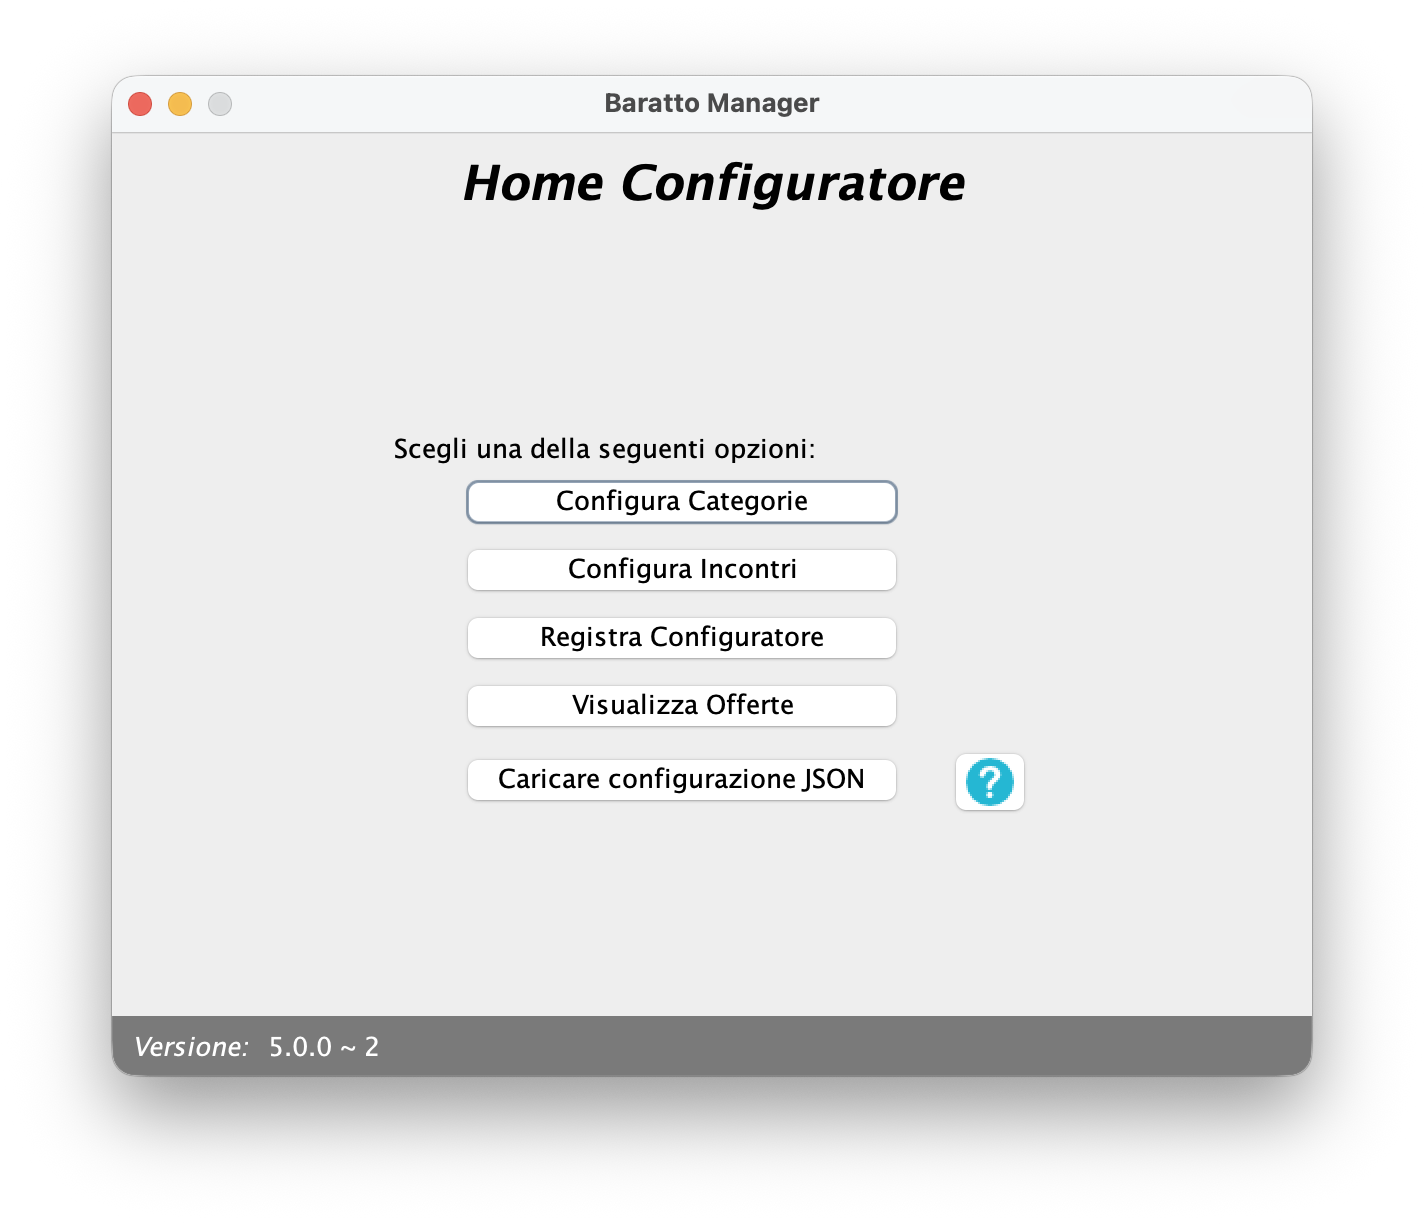
\includegraphics[width=0.5\linewidth]{figures/ss_UI_vecchia/Admin/HomeConfiguratore.png}
    \caption{Homepage del Configuratore}
\end{figure}

\subsection{Costruire il Catalogo}
Il configuratore vede una schermata ad albero che gli permette di creare e gestire le varie categorie e sotto-categorie.
Ad esempio, crea la categoria principale "Elettronica", e al suo interno le sotto-categorie "Computer" e "Smartphone".

\begin{figure}[H]
    \centering
    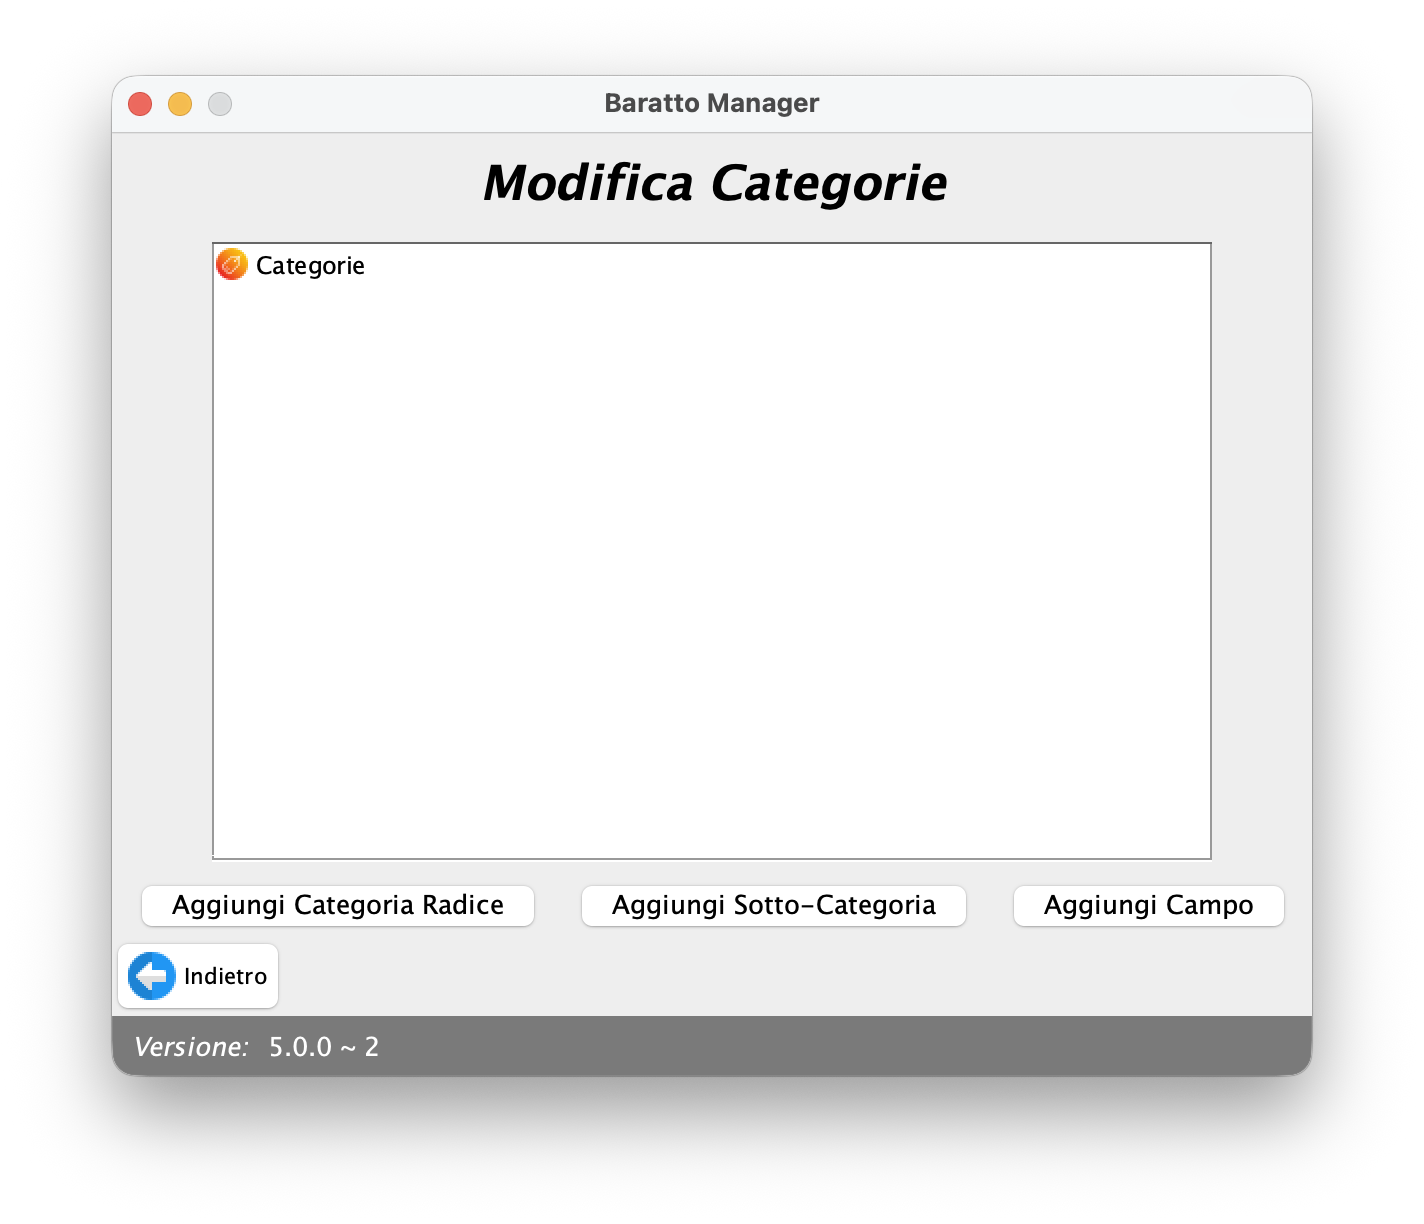
\includegraphics[width=0.5\linewidth]{figures/ss_UI_vecchia/Admin/ModificaCategorie.png}
    \caption{Modifica Categorie (Cofiguratore)}
\end{figure}

\subsubsection{Creazione di una categoria radice}
Il configuratore può definire una categoria radice ovvero una categoria che raccoglie oggetti con caratteristiche comuni. Nell'esempio sopracitato la categoria "Elettronica" è una categoria radice che raggruppa prodotti tecnologici.

\begin{figure}[H]
    \centering
    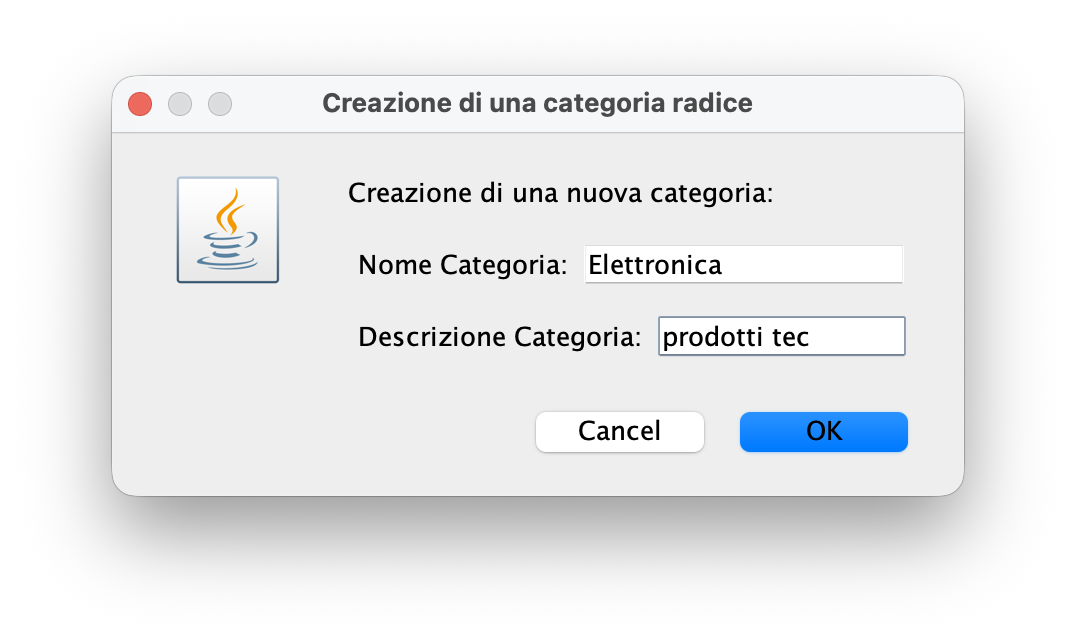
\includegraphics[width=0.5\linewidth]{figures/ss_UI_vecchia/Admin/AggiungiCategoriaRadice.png}
    \caption{Creazione di una categoria radice}
\end{figure}

\subsubsection{Creazione di una sotto-categoria}
Il configuratore, inoltre, deve aggiungere almeno una sotto-categoria per ogni nodo radice. Le sotto-categorie possono essere applicate in modo ricorsivo ad altre sotto-categorie per creare una struttura ad albero complessa. Questa possibiltà permette di andare a settorizzare maggiormente i prodotti.

\begin{multicols*}{2}
    \begin{figure}[H]
        \centering
        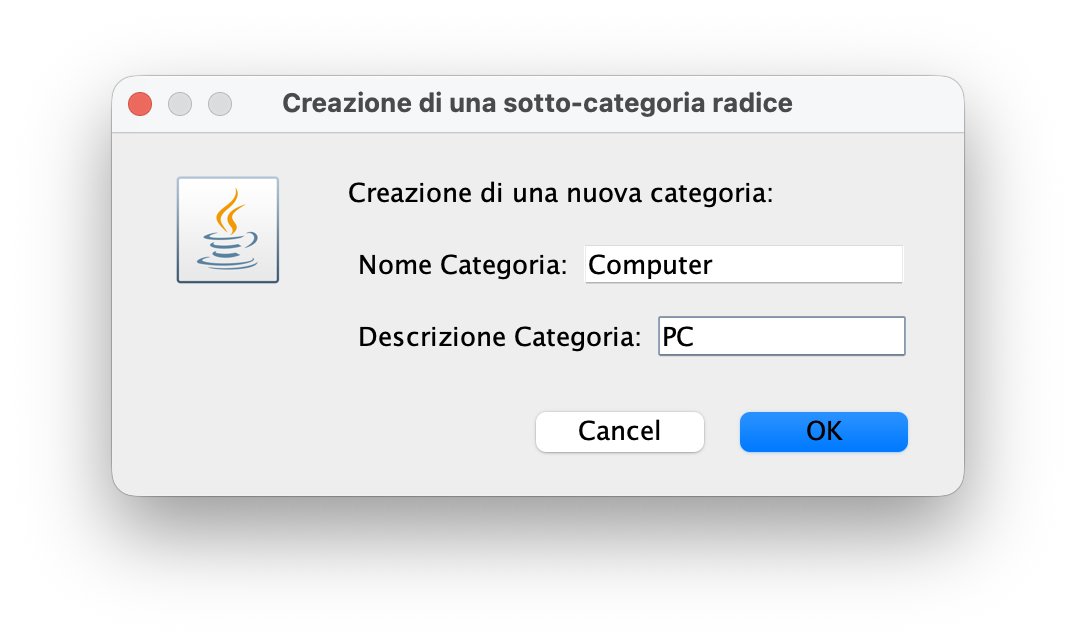
\includegraphics[width=\linewidth]{figures/ss_UI_vecchia/Admin/CreazioneSottocategoria.png}
        \caption{Creazione di una sotto-categoria}
    \end{figure}
    \columnbreak
    \begin{figure}[H]
        \centering
        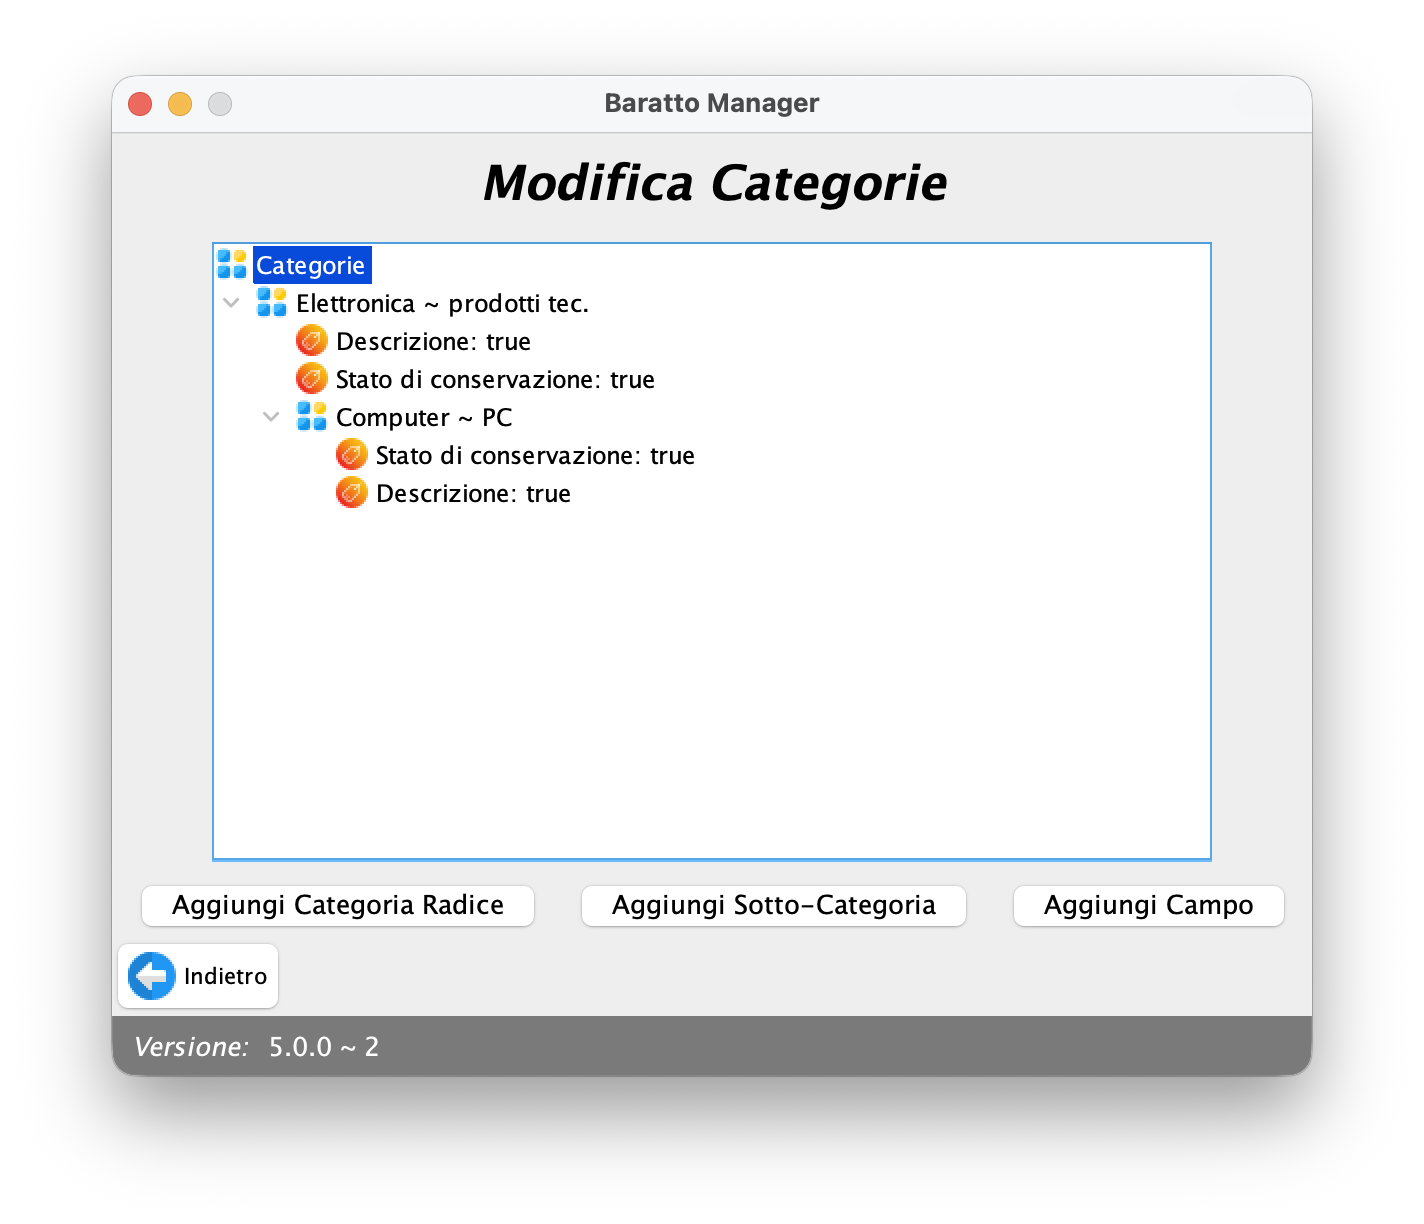
\includegraphics[width=\linewidth]{figures/ss_UI_vecchia/Admin/AlberoCategorie.png}
        \caption{Visualizzazione albero delle\\categorie (Configuratore)}
    \end{figure}
\end{multicols*}

\subsubsection{Definire i Campi}
Per dare la possibilità agli utenti di specificare più dettagli per una determinata sotto-categoria vengono messi a disposizione dal configuratore dei campi, che possono essere obligatori o meno.

Ad esempio, per la sotto-categoria "Computer", imposterà che chiunque voglia caricare un dispositivo dovrà obbligatoriamente compilare i campi "Modello", "Marca", "Descrizione" e "Stato"; mentre il campo "Colore" è facoltativo.

\begin{multicols*}{2}
    \begin{figure}[H]
        \centering
        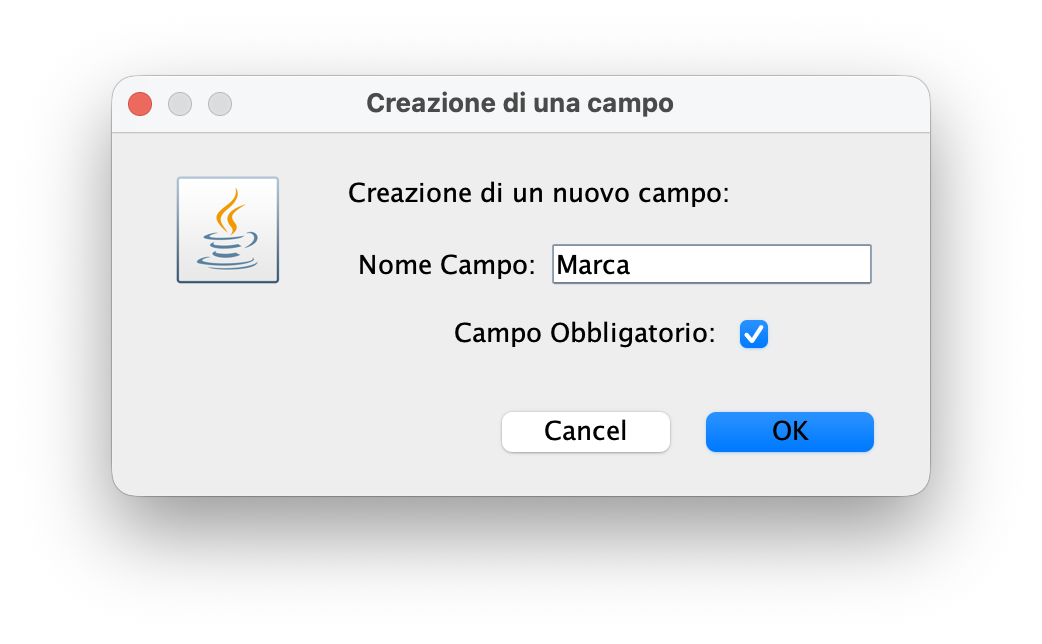
\includegraphics[width=\linewidth]{figures/ss_UI_vecchia/Admin/CreazioneCampo.png}
        \caption{Creazione di un nuovo campo}
    \end{figure}
    \columnbreak
    \begin{figure}[H]
        \centering
        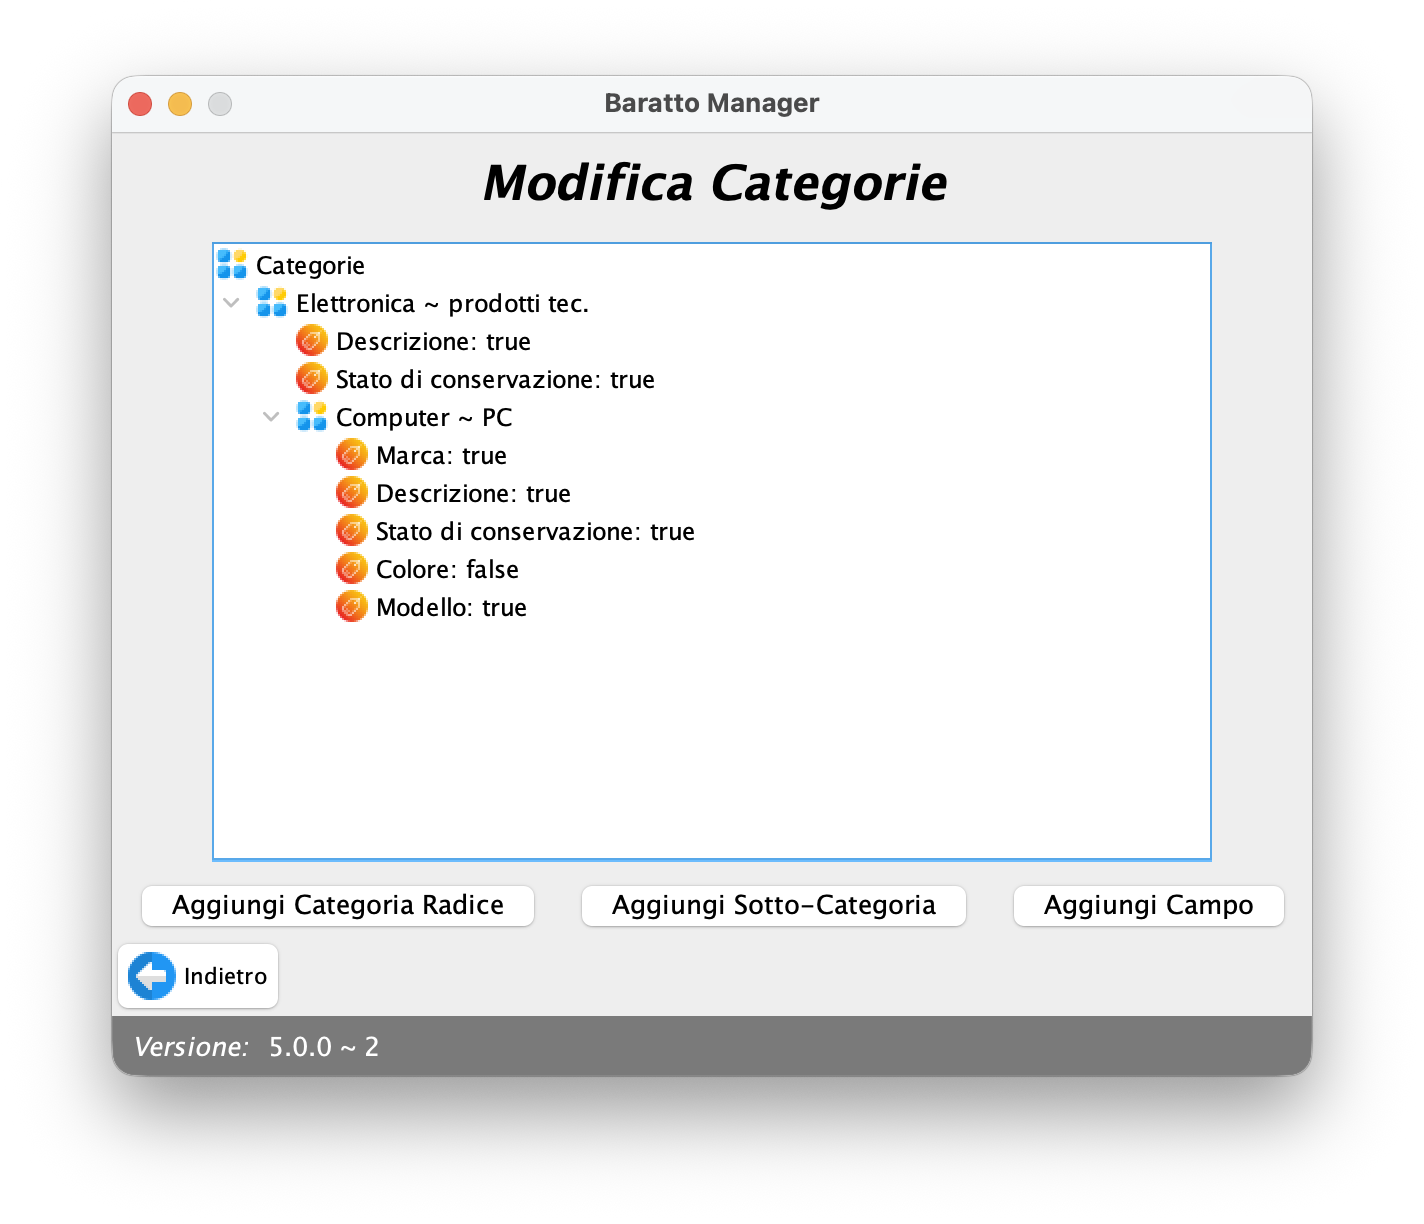
\includegraphics[width=\linewidth]{figures/ss_UI_vecchia/Admin/ModificaCategoriaCompleto.png}
        \caption{Visualizzazione albero delle\\categorie con tutti i campi}
    \end{figure}
\end{multicols*}

\subsection{Creare i Luoghi di Incontro}
Poiché lo scambio finale è fisico, il configuratore imposta una bacheca di appuntamenti organizzati.

Tramite un apposito modulo, crea dei luoghi e orari disponibili. Es: "Milano, Piazza Duomo, tutti i Giovedì dalle 15:00 alle 17:00, con 4 giorni di tempo per confermare lo scambio".

\begin{multicols*}{2}
    \begin{figure}[H]
        \centering
        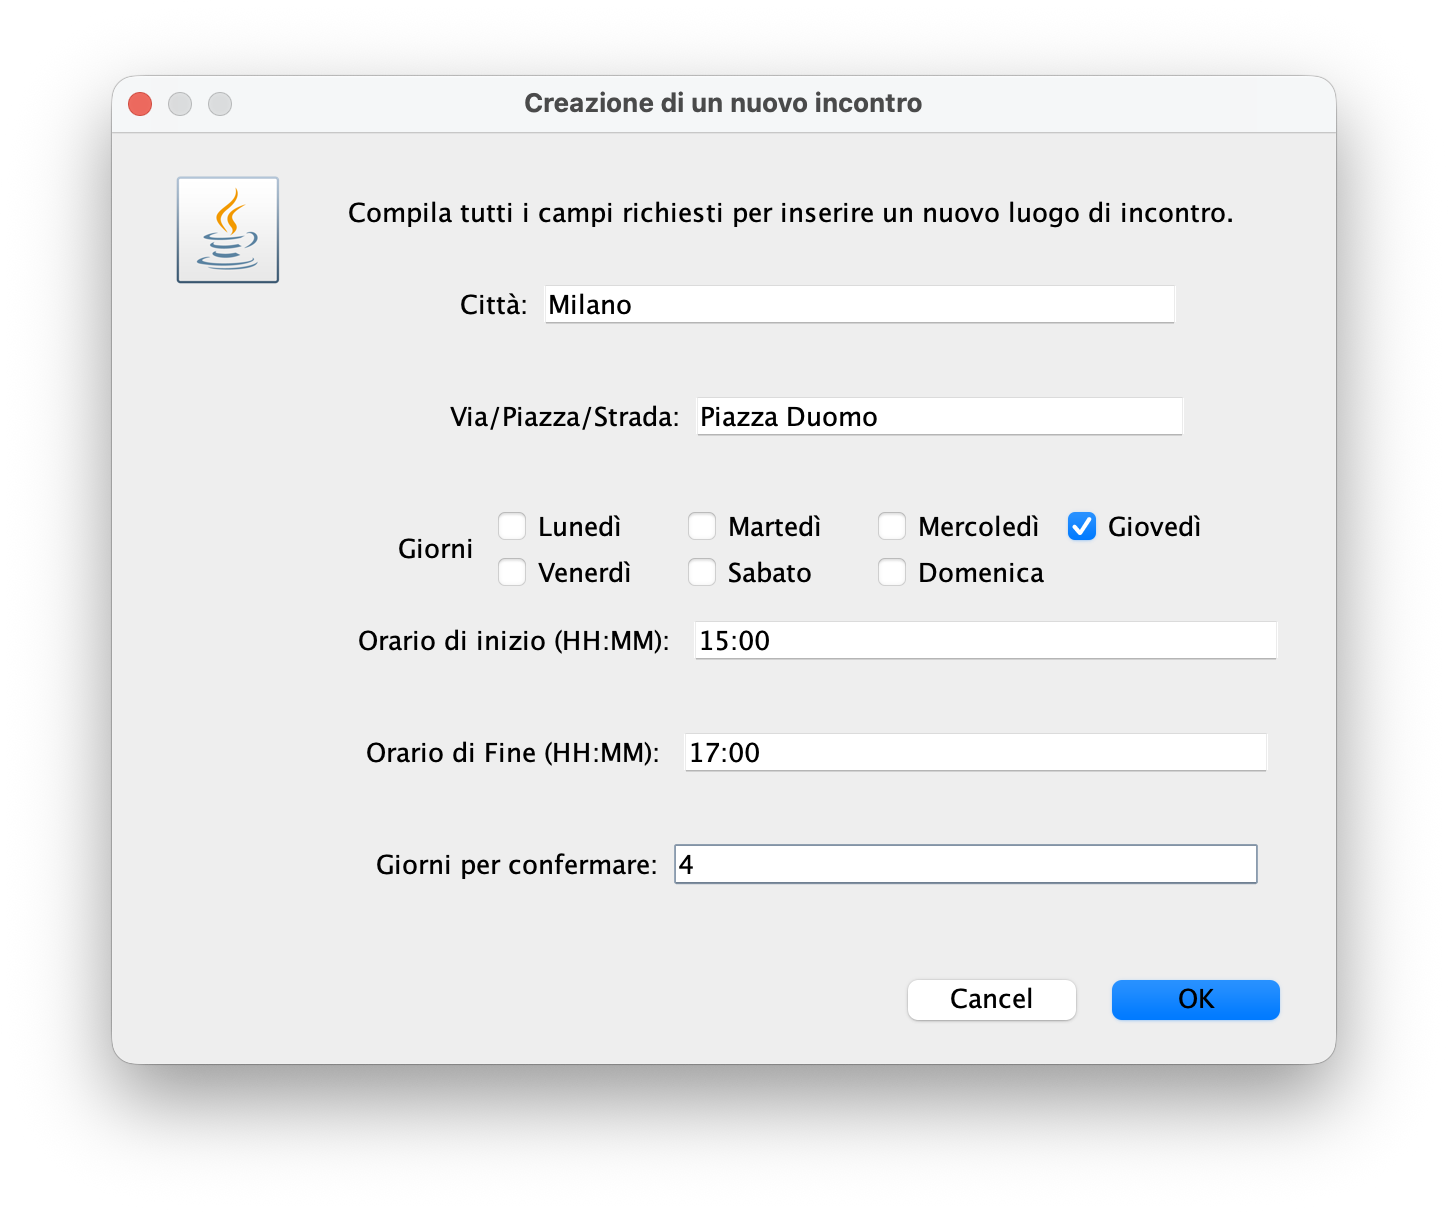
\includegraphics[width=\linewidth]{figures/ss_UI_vecchia/Admin/CreazioneIncontro.png}
        \caption{Creazione di un nuovo incontro}
    \end{figure}
    \columnbreak
    \begin{figure}[H]
        \centering
        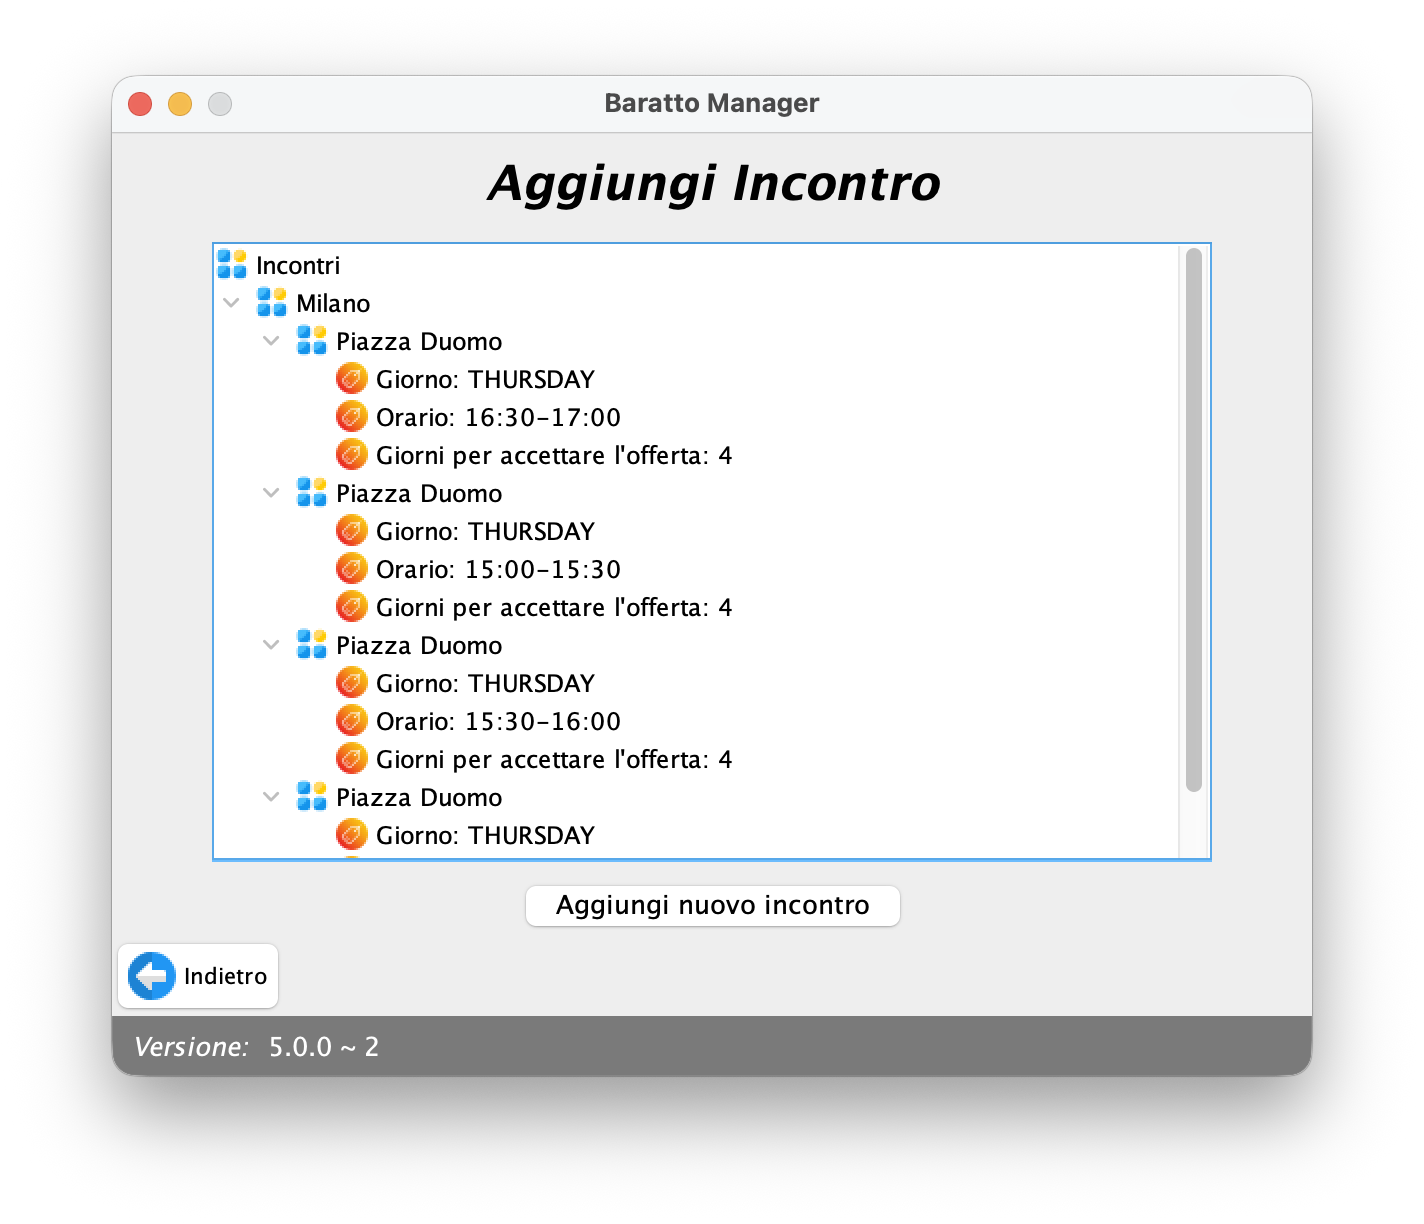
\includegraphics[width=\linewidth]{figures/ss_UI_vecchia/Admin/IncontroAggiunto.png}
        \caption{Visualizzazione ad albero degli incotri}
    \end{figure}
\end{multicols*}

\subsection{Altre funzionalità}

\subsubsection{Registrare nuovi configuratori}
Il configuratore può registrare altri account "\textit{configuratori}" inserendo un nome utente univoco a cui viene abbinata una password di default ("\textit{123}") che dovrà essere modificata al primo accesso.

\begin{figure}[H]
    \centering
    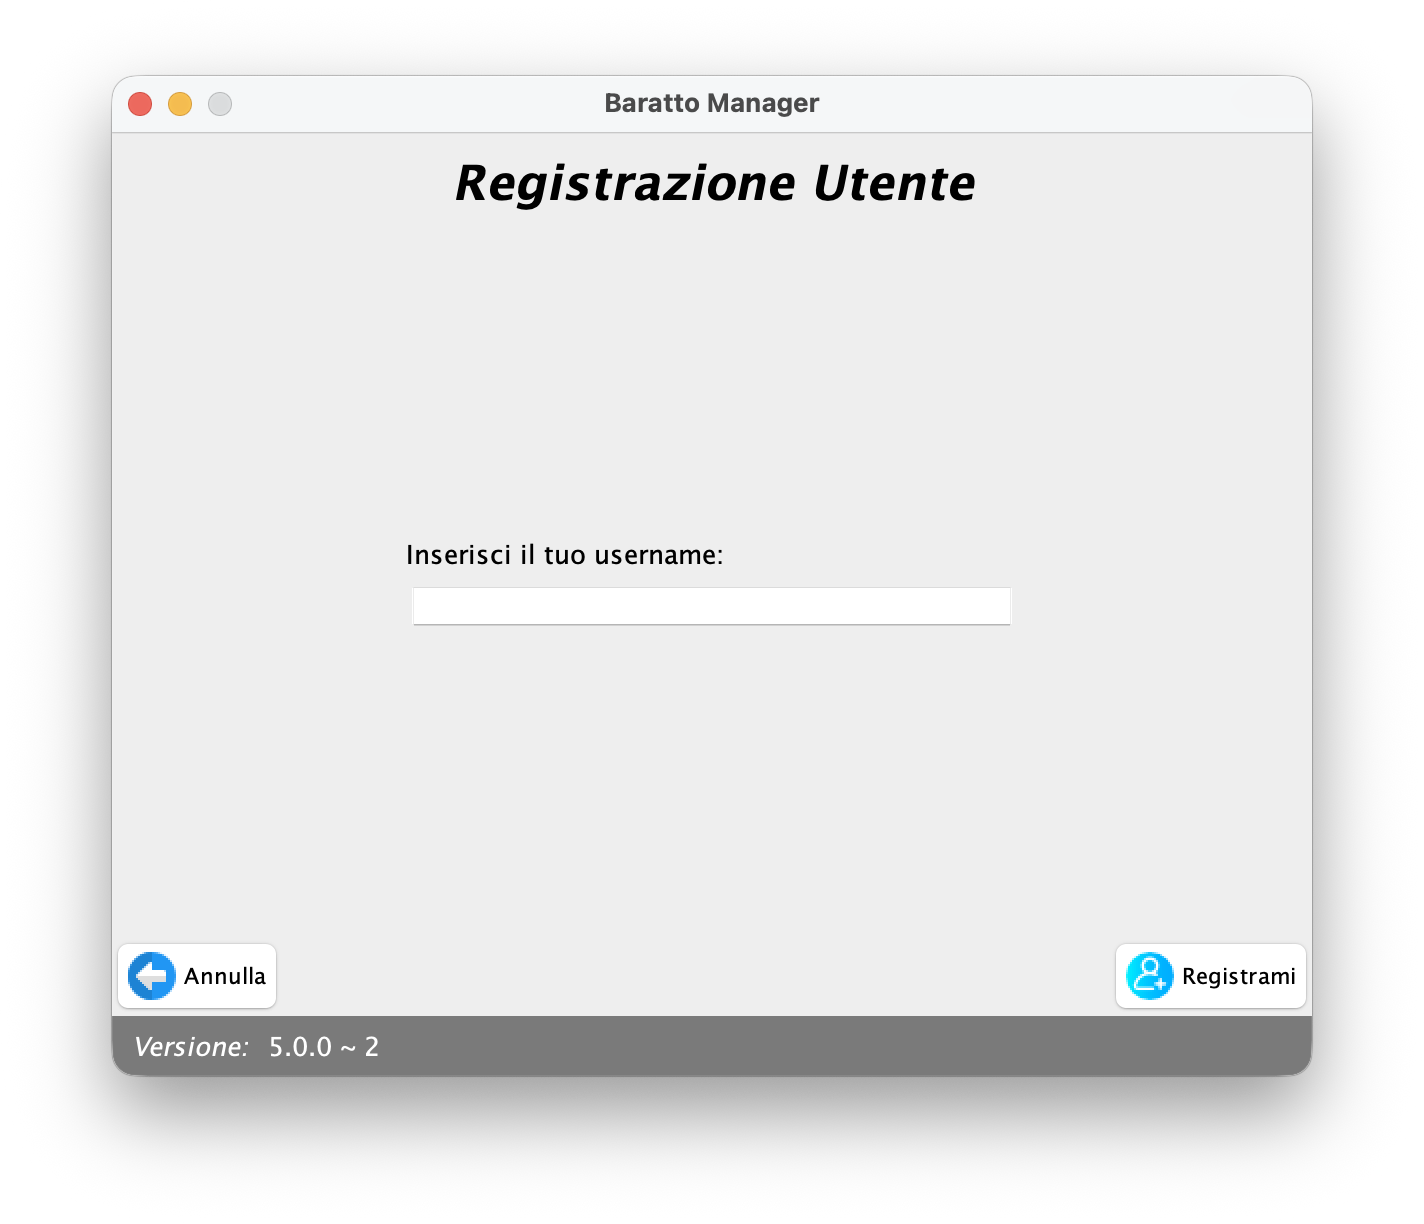
\includegraphics[width=0.5\linewidth]{figures/ss_UI_vecchia/Admin/RegistrazioneNuovoConfiguratore.png}
    \caption{Registrazione di un nuovo account configuratore}
\end{figure}

\subsubsection{Visualizzare le offerte}
Il configuratore può visualizzare lo stato degli scambi in corso e chiusi.

\begin{multicols*}{2}
    \begin{figure}[H]
        \centering
        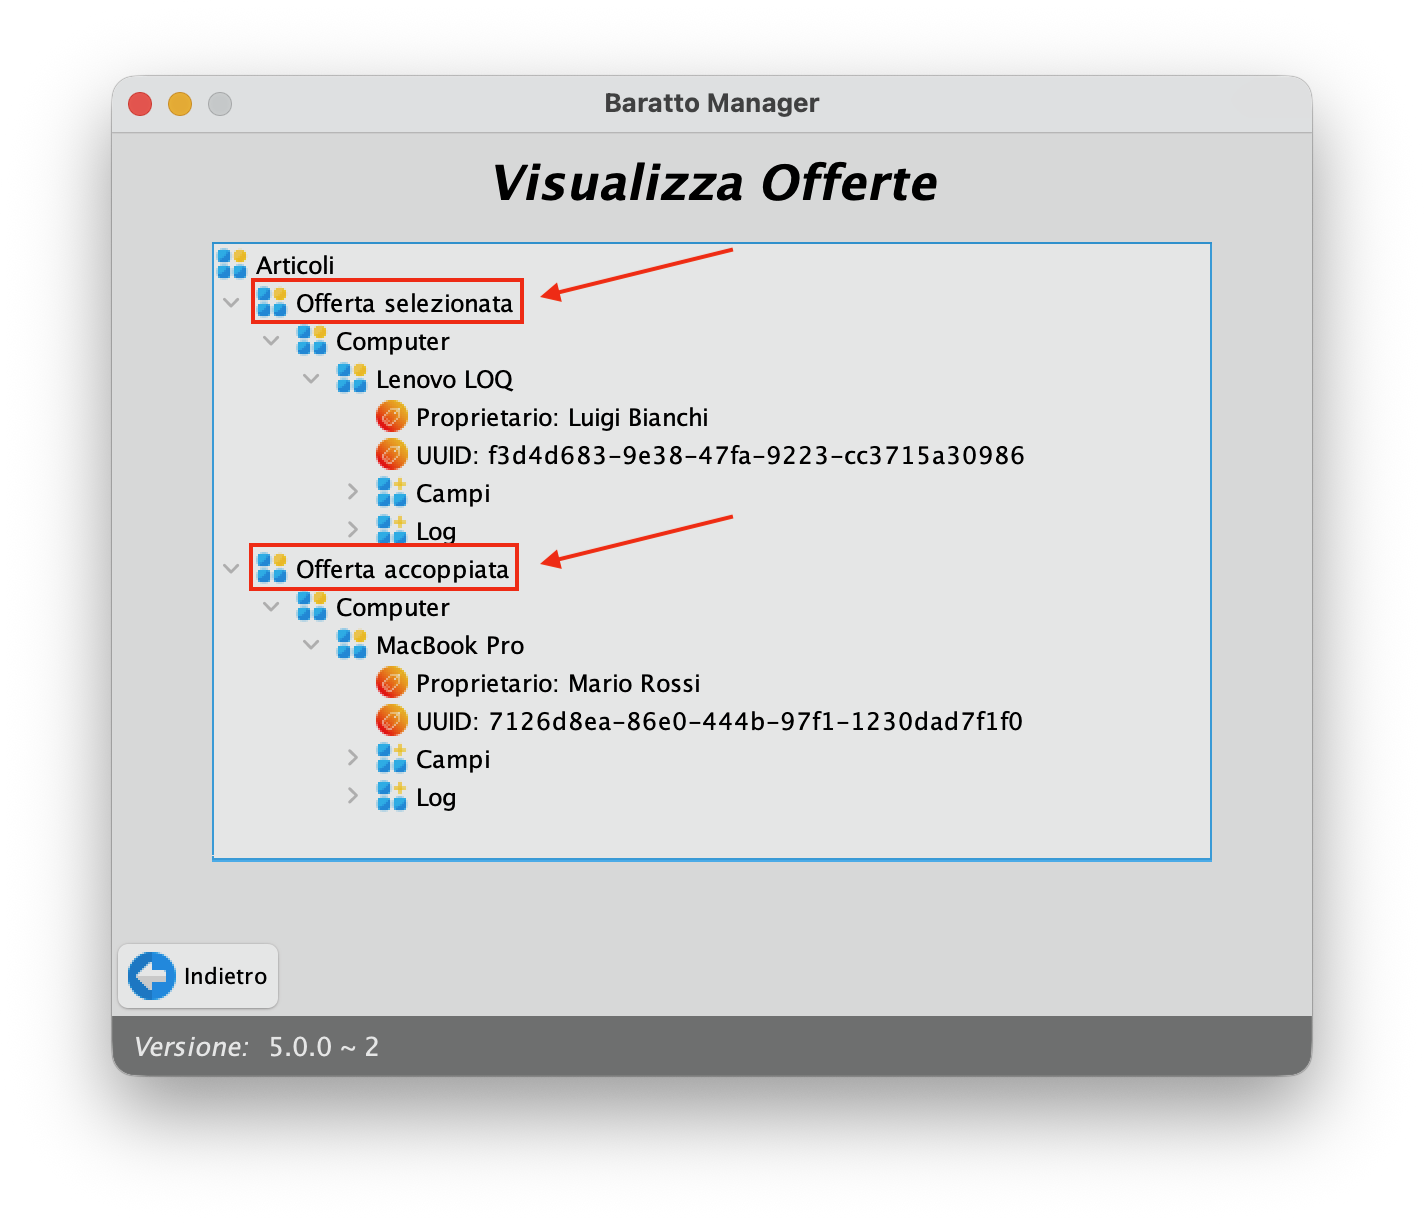
\includegraphics[width=\linewidth]{figures/ss_UI_vecchia/Admin/OfferteAperte.png}
        \caption{Visualizzazione scambi aperti}
    \end{figure}
    \columnbreak
    \begin{figure}[H]
        \centering
        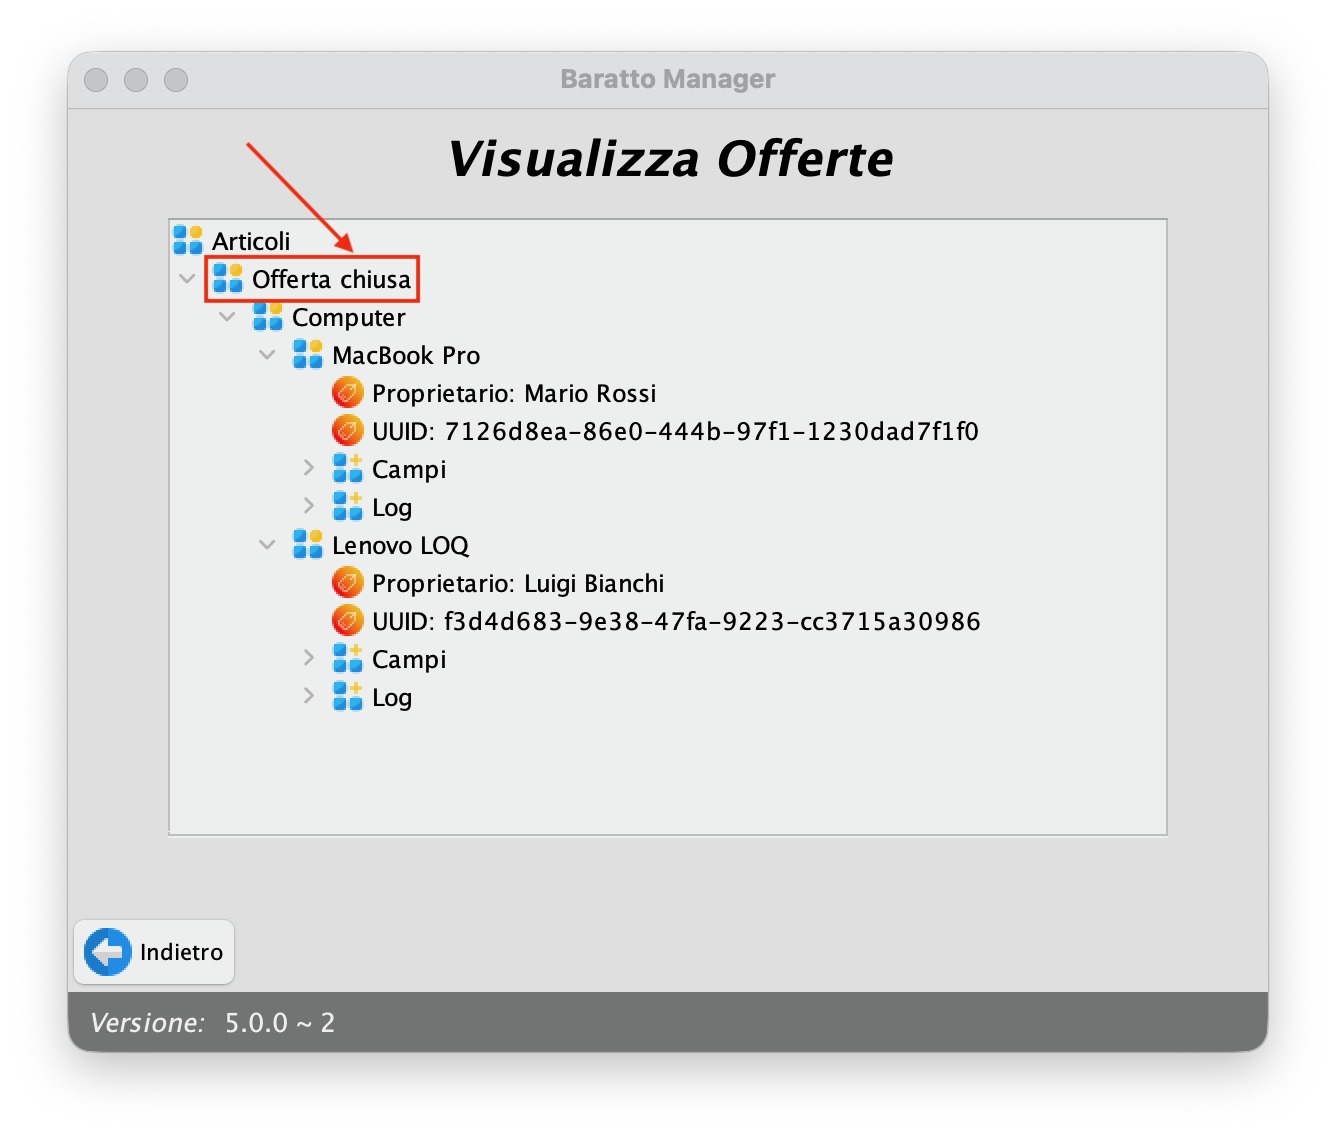
\includegraphics[width=\linewidth]{figures/ss_UI_vecchia/Admin/OfferteChiuse.png}
        \caption{Visualizzazione scambi conclusi}
    \end{figure}
\end{multicols*}

\subsubsection{Caricare una configurazione}
Il configuratore può caricare un file JSON che contiene una configurazione di partenza. Vengono importate in un'unica operazione categorie, sottocategorie, campi e parametri di configurazione.

Il file JSON deve rispettare un formato standard corrispondente a quello definito all'interno dell'help e rifiuta i file con errori.
\begin{figure}[H]
    \centering
    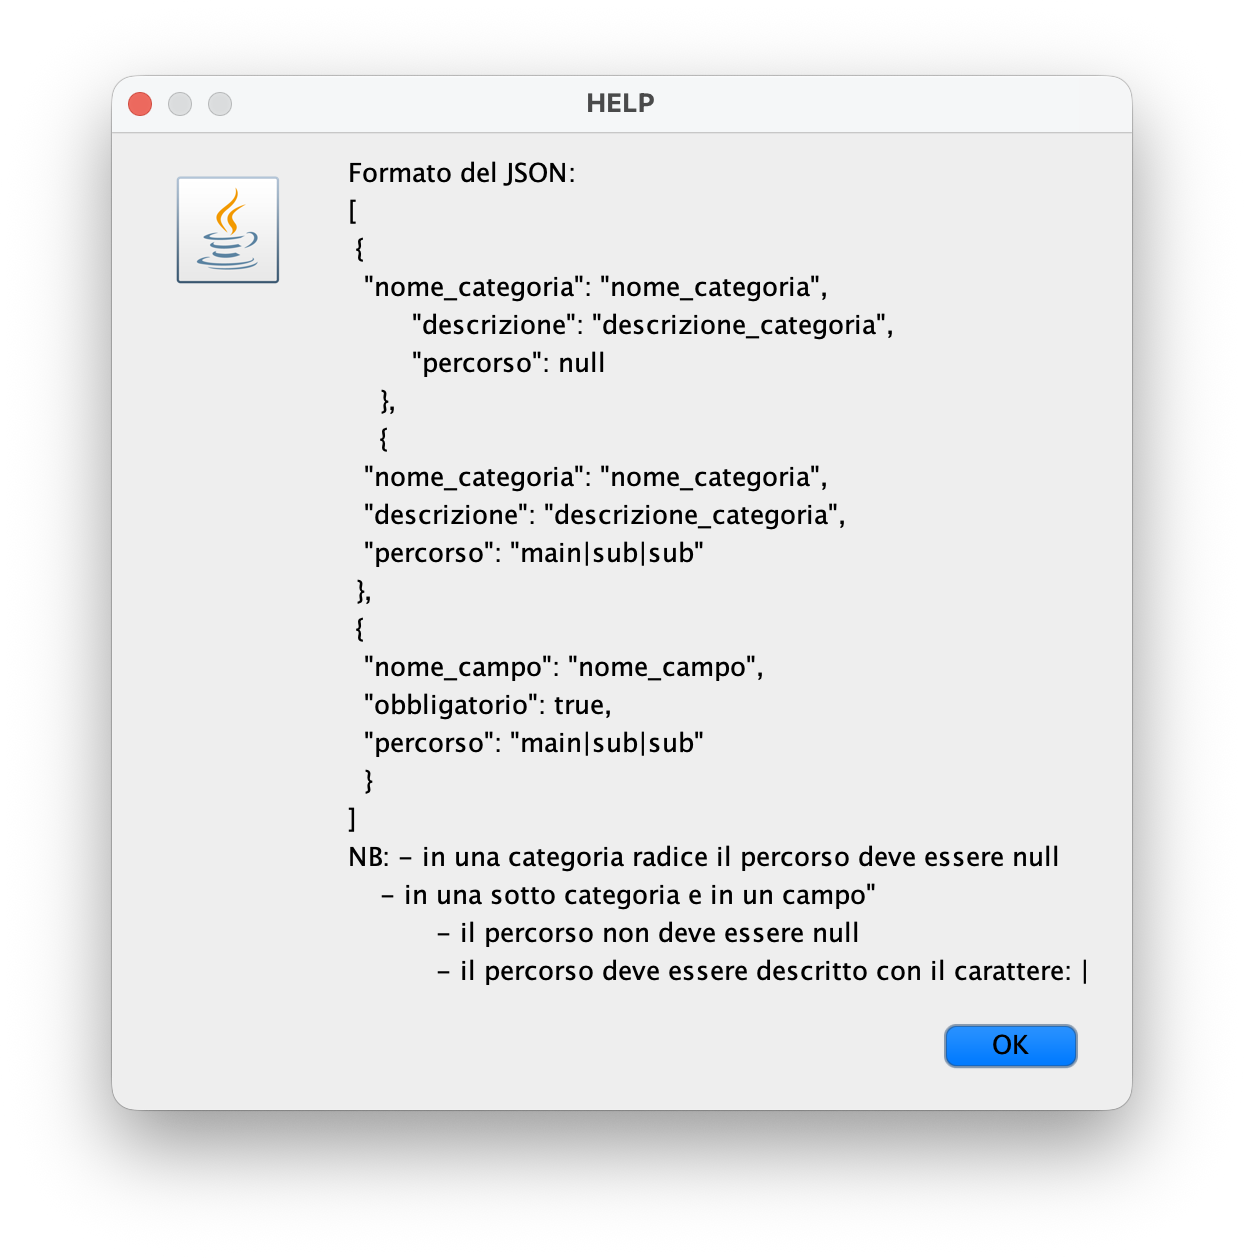
\includegraphics[width=0.5\linewidth]{figures/ss_UI_vecchia/Admin/CaricareJSON.png}
    \caption{Formato JSON dei dati da caricare.}
\end{figure}

\section{L'area del Fruitore}
Ll fruitore può consultare l'elenco delle categorie con relative sottocategorie e campi, e l'elenco dei luoghi di incontro con giorni e orari per poter effettuare gli scambi.

\begin{figure}[H]
    \centering
    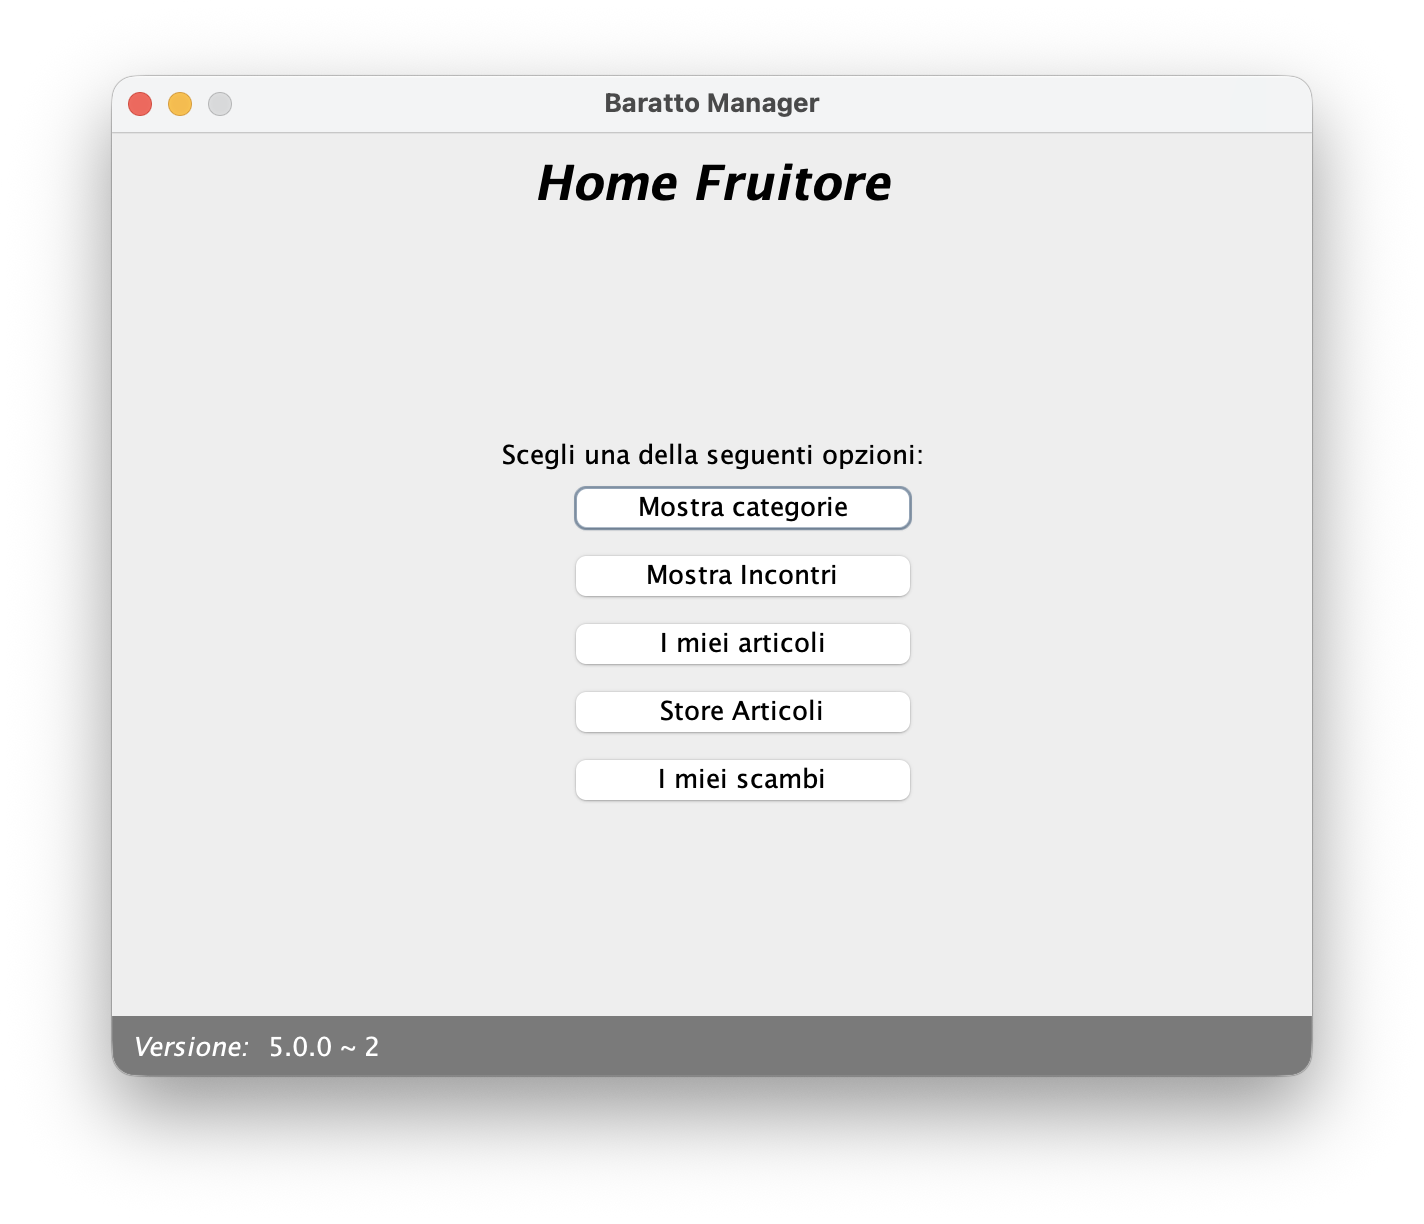
\includegraphics[width=0.5\linewidth]{figures/ss_UI_vecchia/Utente/HomeUtente.png}
    \caption{Homapage del Fruitore}
\end{figure}

\subsection{Funzionalità di visualizzazione}
Il fruitore può vedere l'albero della categorie e quello degli incontri. Lo schema di visualizzazione è analogo a quello dei configuratori, senza però le funzionalità di aggiunta.

\begin{multicols*}{2}
    \begin{figure}[H]
        \centering
        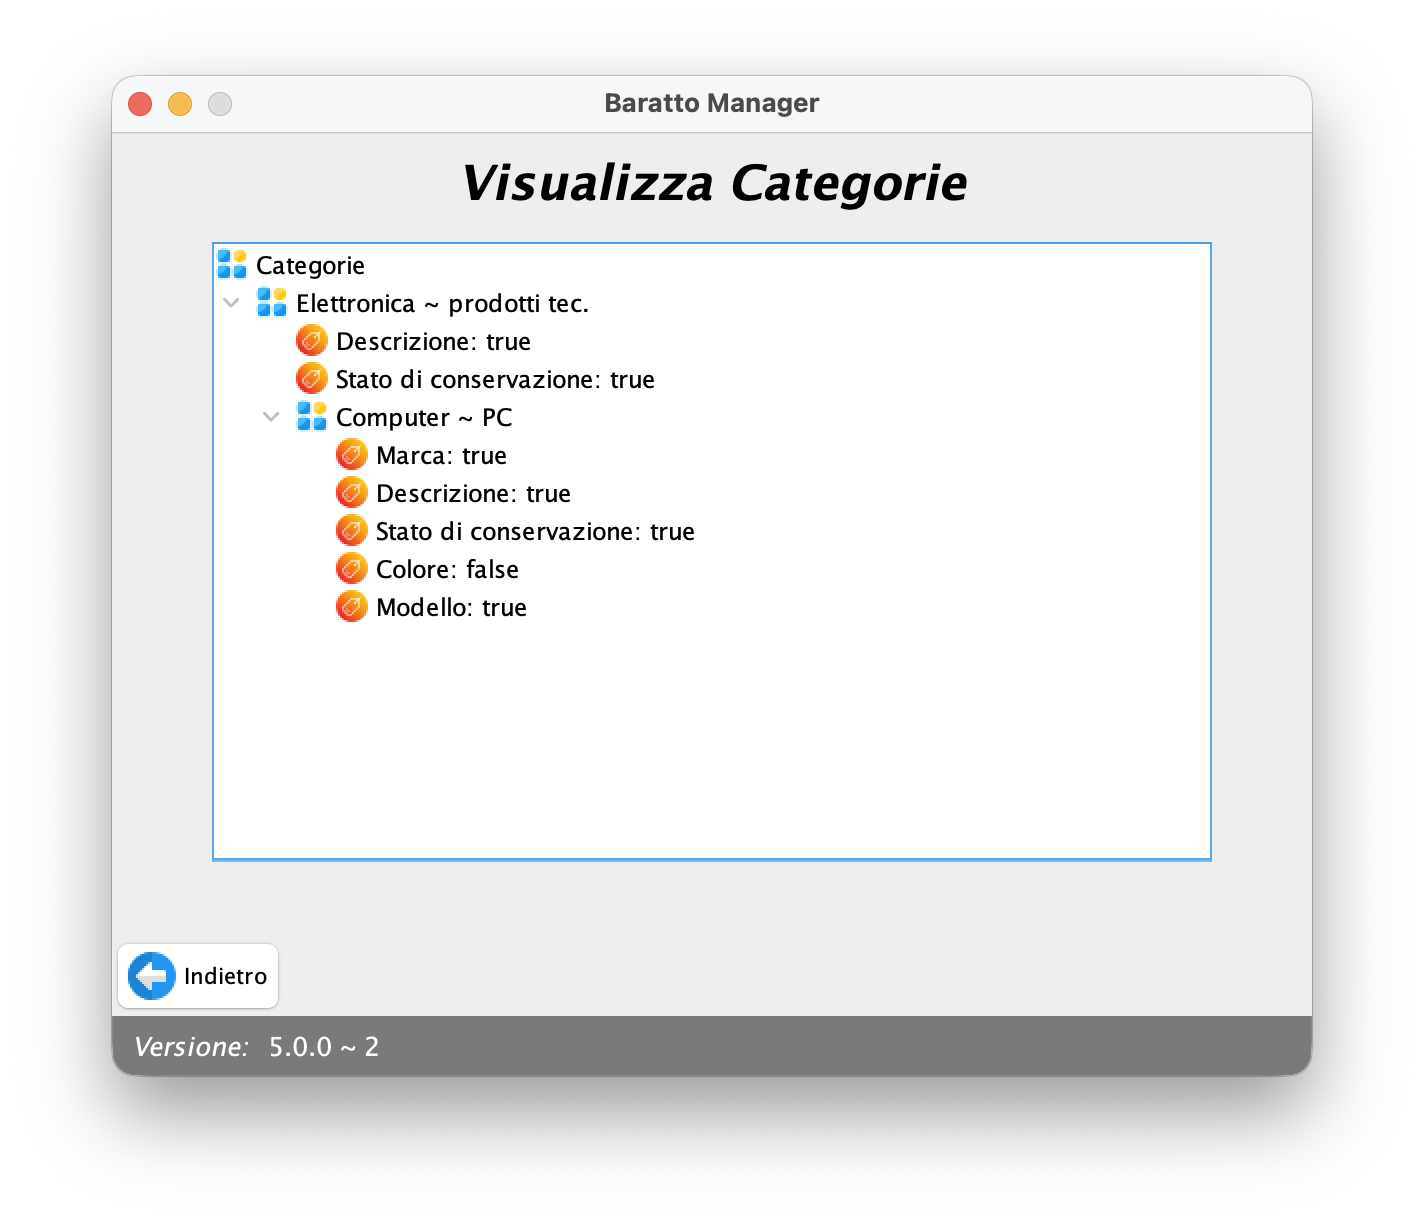
\includegraphics[width=\linewidth]{figures/ss_UI_vecchia/Utente/VisualizzazioneCategorie.png}
        \caption{Visualizzazione dell'albero delle categorie}
    \end{figure}
    \columnbreak
    \begin{figure}[H]
        \centering
        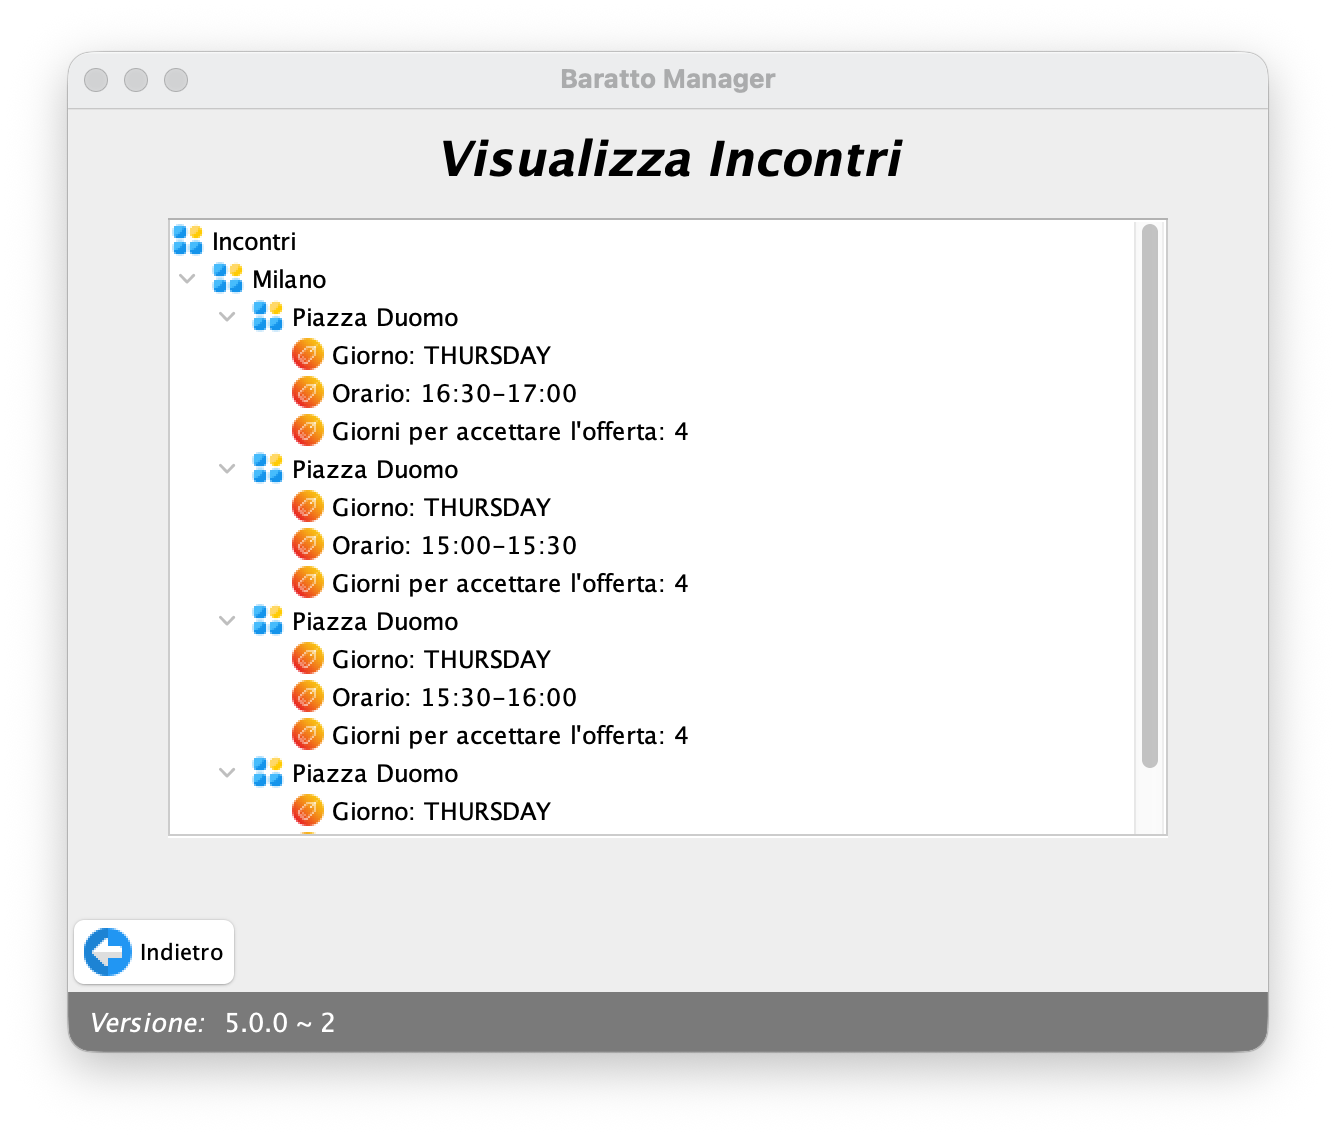
\includegraphics[width=\linewidth]{figures/ss_UI_vecchia/Utente/VisualizzazioneIncontri.png}
        \caption{Visualizzazione dell'albero degli incotri}
    \end{figure}
\end{multicols*}

\subsection{Aggiunta dei propri articoli}
Il fruitore può caricare i proprio articoli selezionando la categoria di appartenenza e compilando il modulo delle informazioni.
\begin{multicols*}{2}
    \begin{figure}[H]
        \centering
        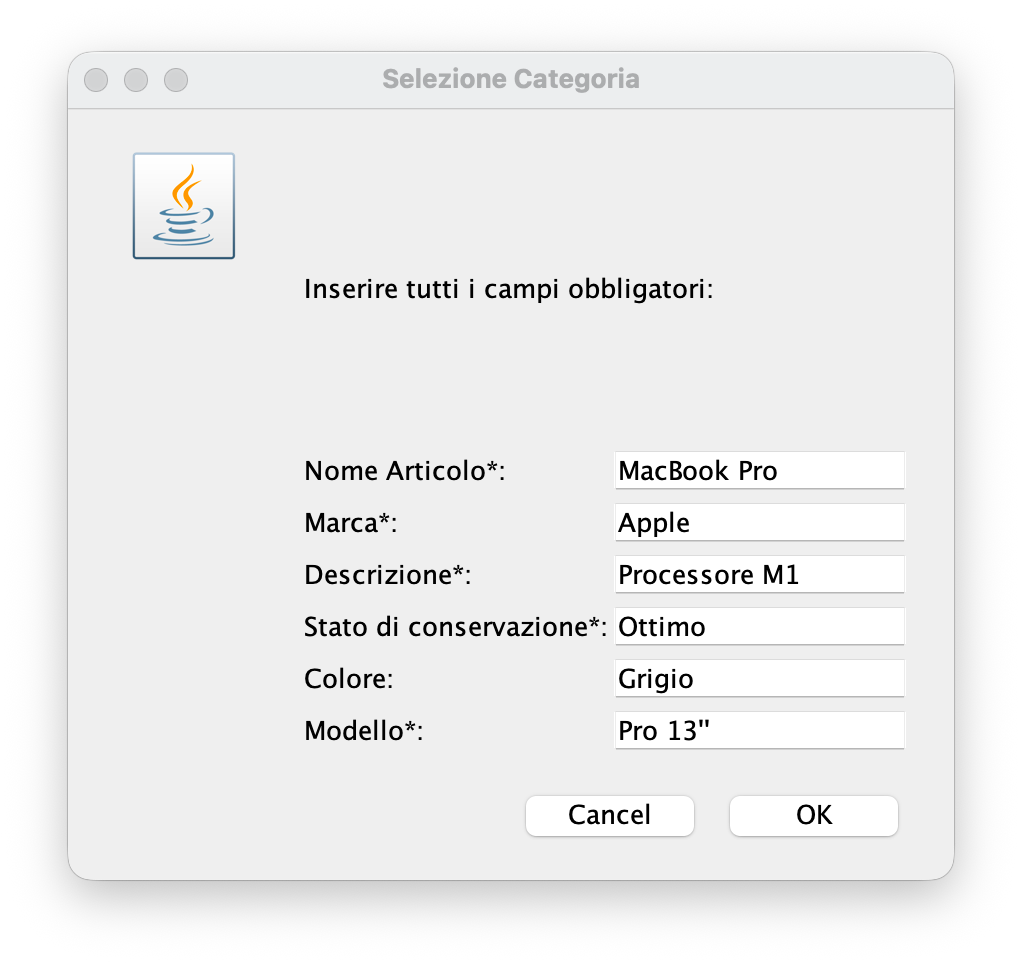
\includegraphics[width=\linewidth]{figures/ss_UI_vecchia/Utente/NuovoArticolo.png}
        \caption{Caricamento di un nuovo articolo}
    \end{figure}
    \columnbreak
    \begin{figure}[H]
        \centering
        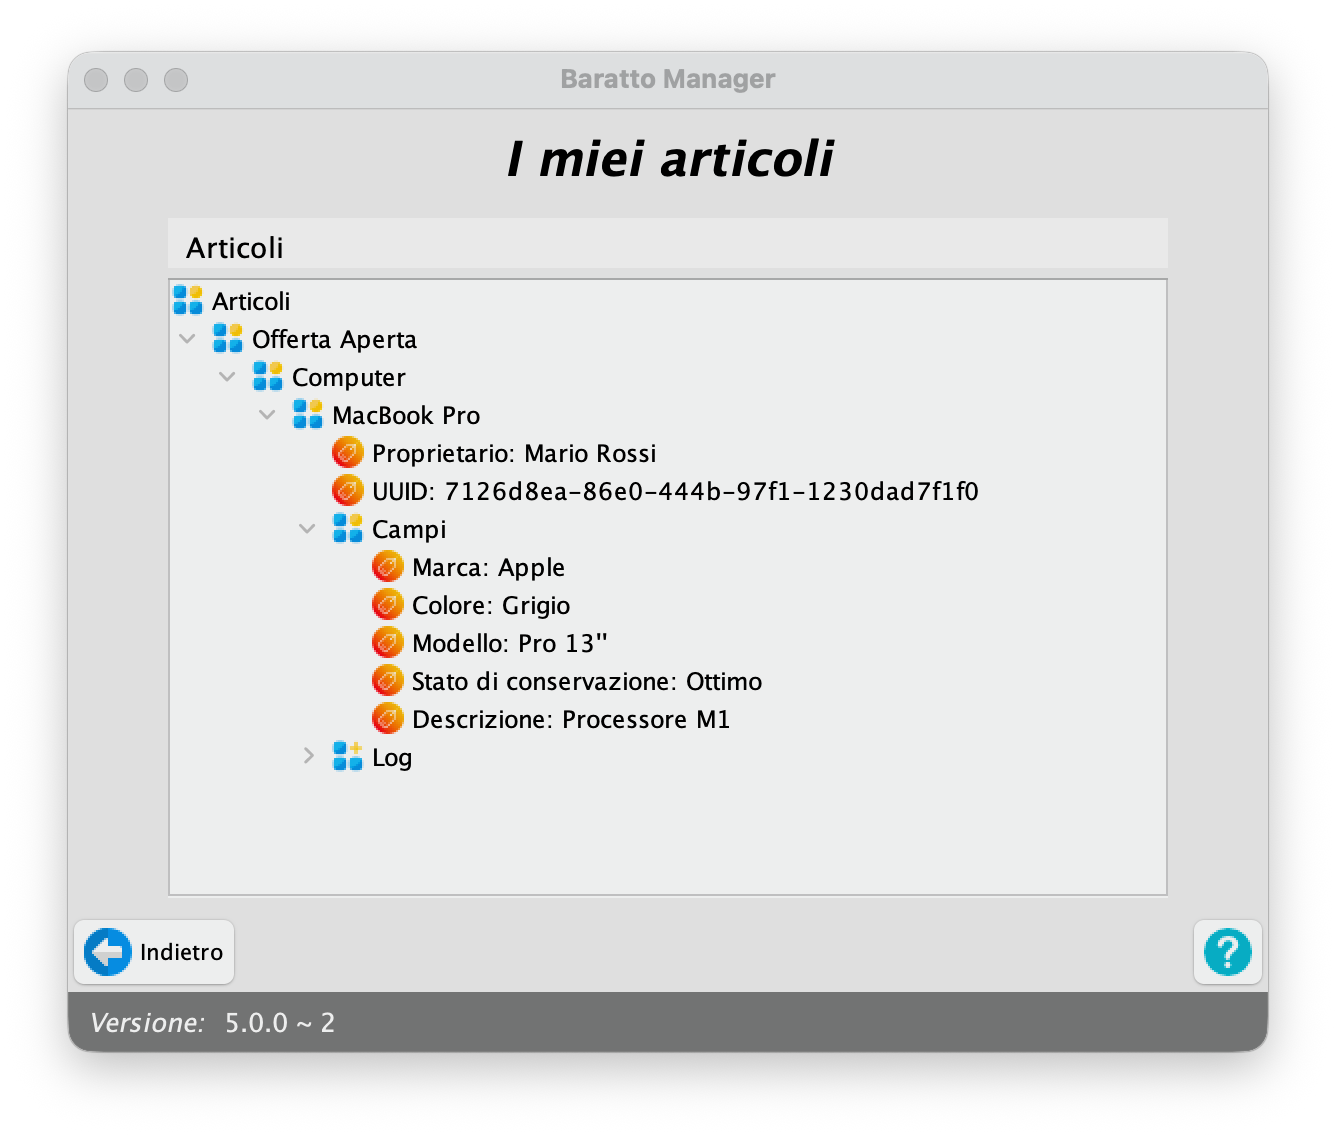
\includegraphics[width=\linewidth]{figures/ss_UI_vecchia/Utente/ArticoliUtente.png}
        \caption{Riepilogo dei propri articoli}
    \end{figure}
\end{multicols*}

\subsection{Scambiare articoli}
Il fruitore visualizza il catalogo degli articoli disponibili, sceglie quello che gli interessa e inizia scambio.
Il sistema fa scegliere un proprio articolo da scambiare e fa selezionare data e luogo di incontro.
\begin{multicols*}{3}
    \begin{figure}[H]
        \centering
        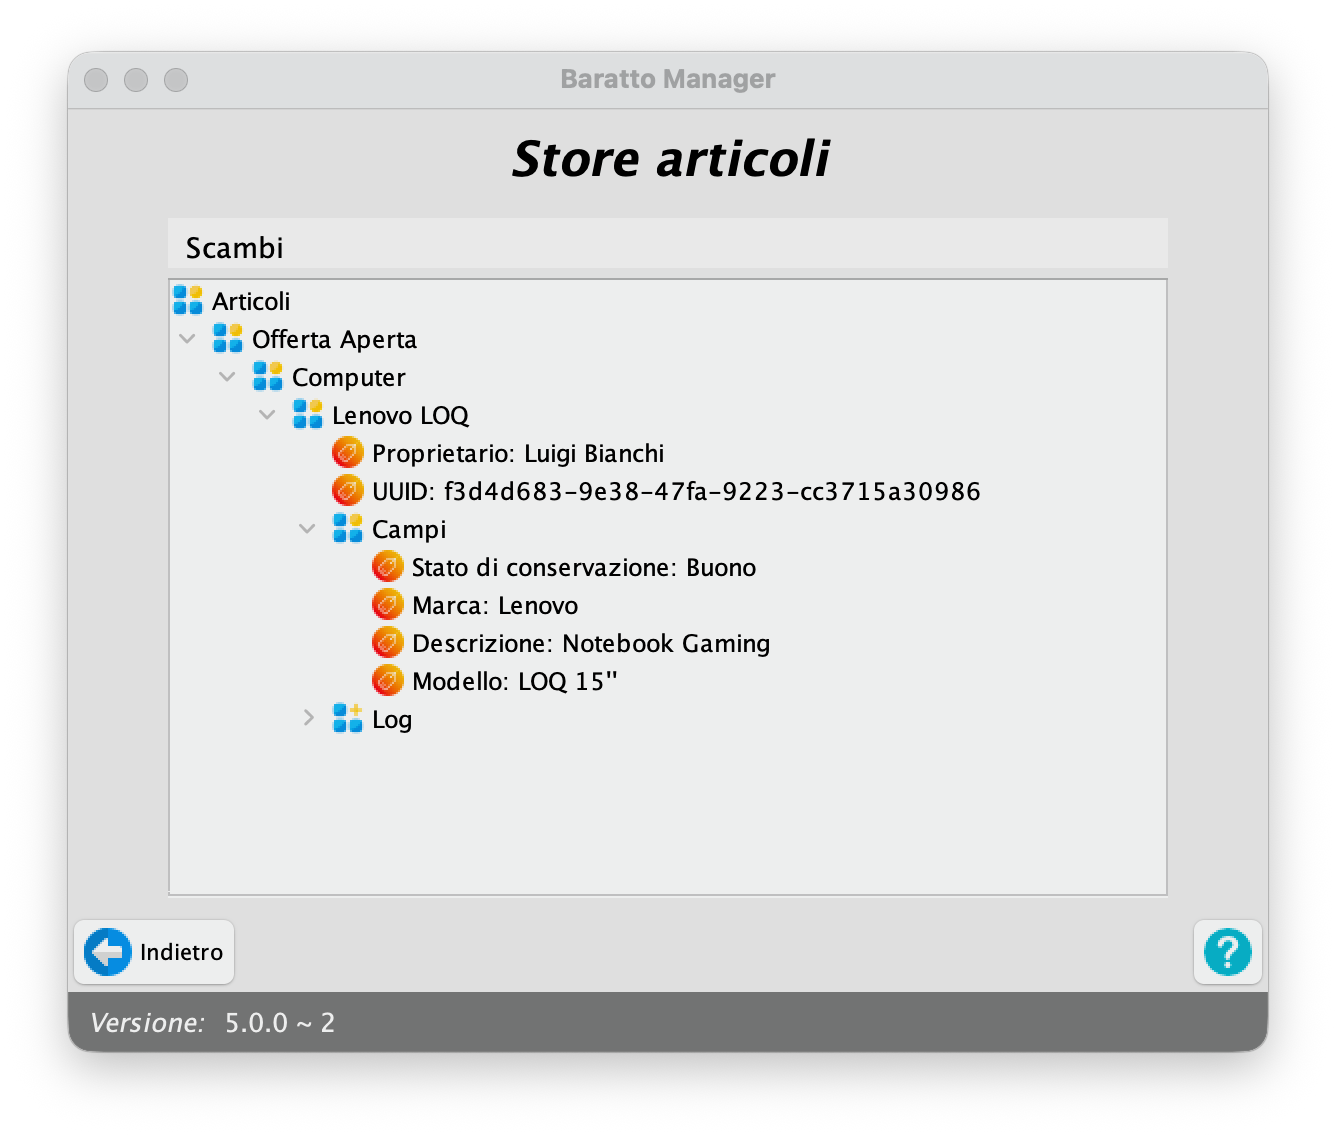
\includegraphics[width=\linewidth]{figures/ss_UI_vecchia/Utente/StoreArticoli.png}
        \caption{Step 1 - Visualizza lo store e seleziona un articolo}
    \end{figure}
    \columnbreak
    \begin{figure}[H]
        \centering
        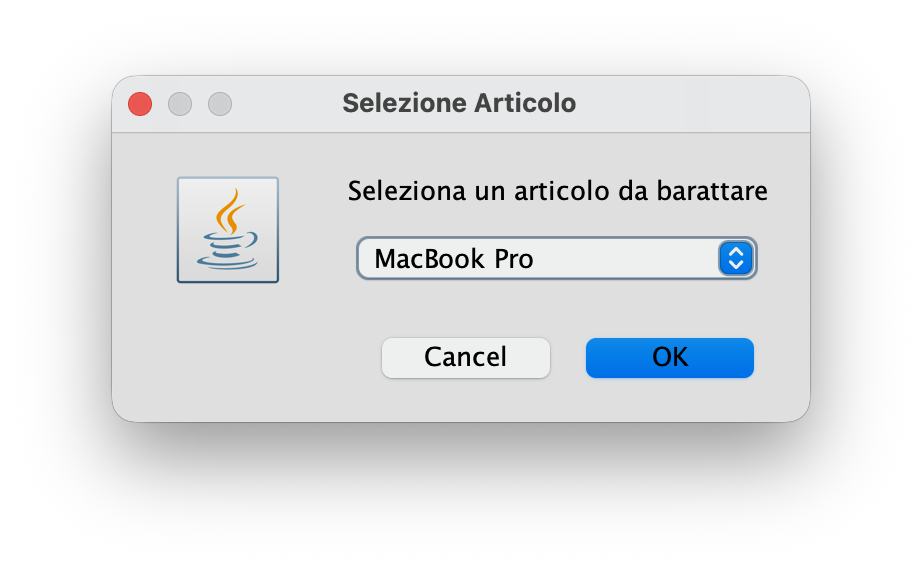
\includegraphics[width=\linewidth]{figures/ss_UI_vecchia/Utente/SelezionaArticolo.png}
        \caption{Step 2 - Sceglie l'articolo da scambiare}
    \end{figure}
    \columnbreak
    \begin{figure}[H]
        \centering
        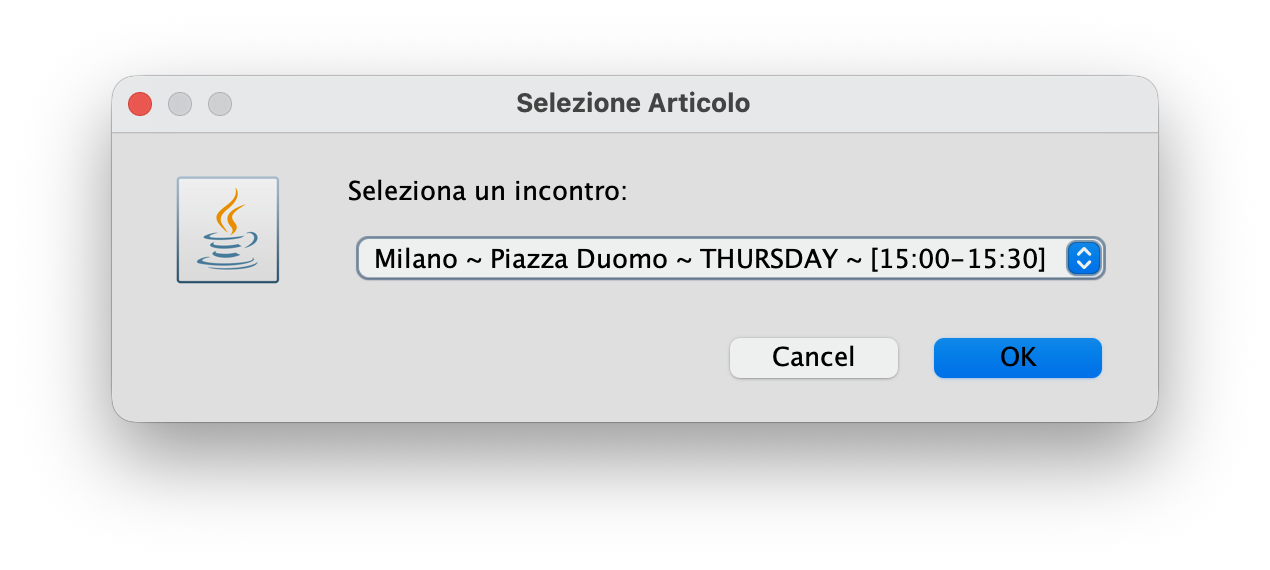
\includegraphics[width=\linewidth]{figures/ss_UI_vecchia/Utente/SelezionaIncontro.png}
        \caption{Step 3 - Scelta incontro}
    \end{figure}
\end{multicols*}

\subsection{Scambi attivi}
In questa pagina l'utente può visualizzare sia gli scambi che attendono risposta, confermandoli o riprogrammando l'incontro, sia quelli confermati (\textit{CLOSED}).
\begin{multicols*}{3}
    \begin{figure}[H]
        \centering
        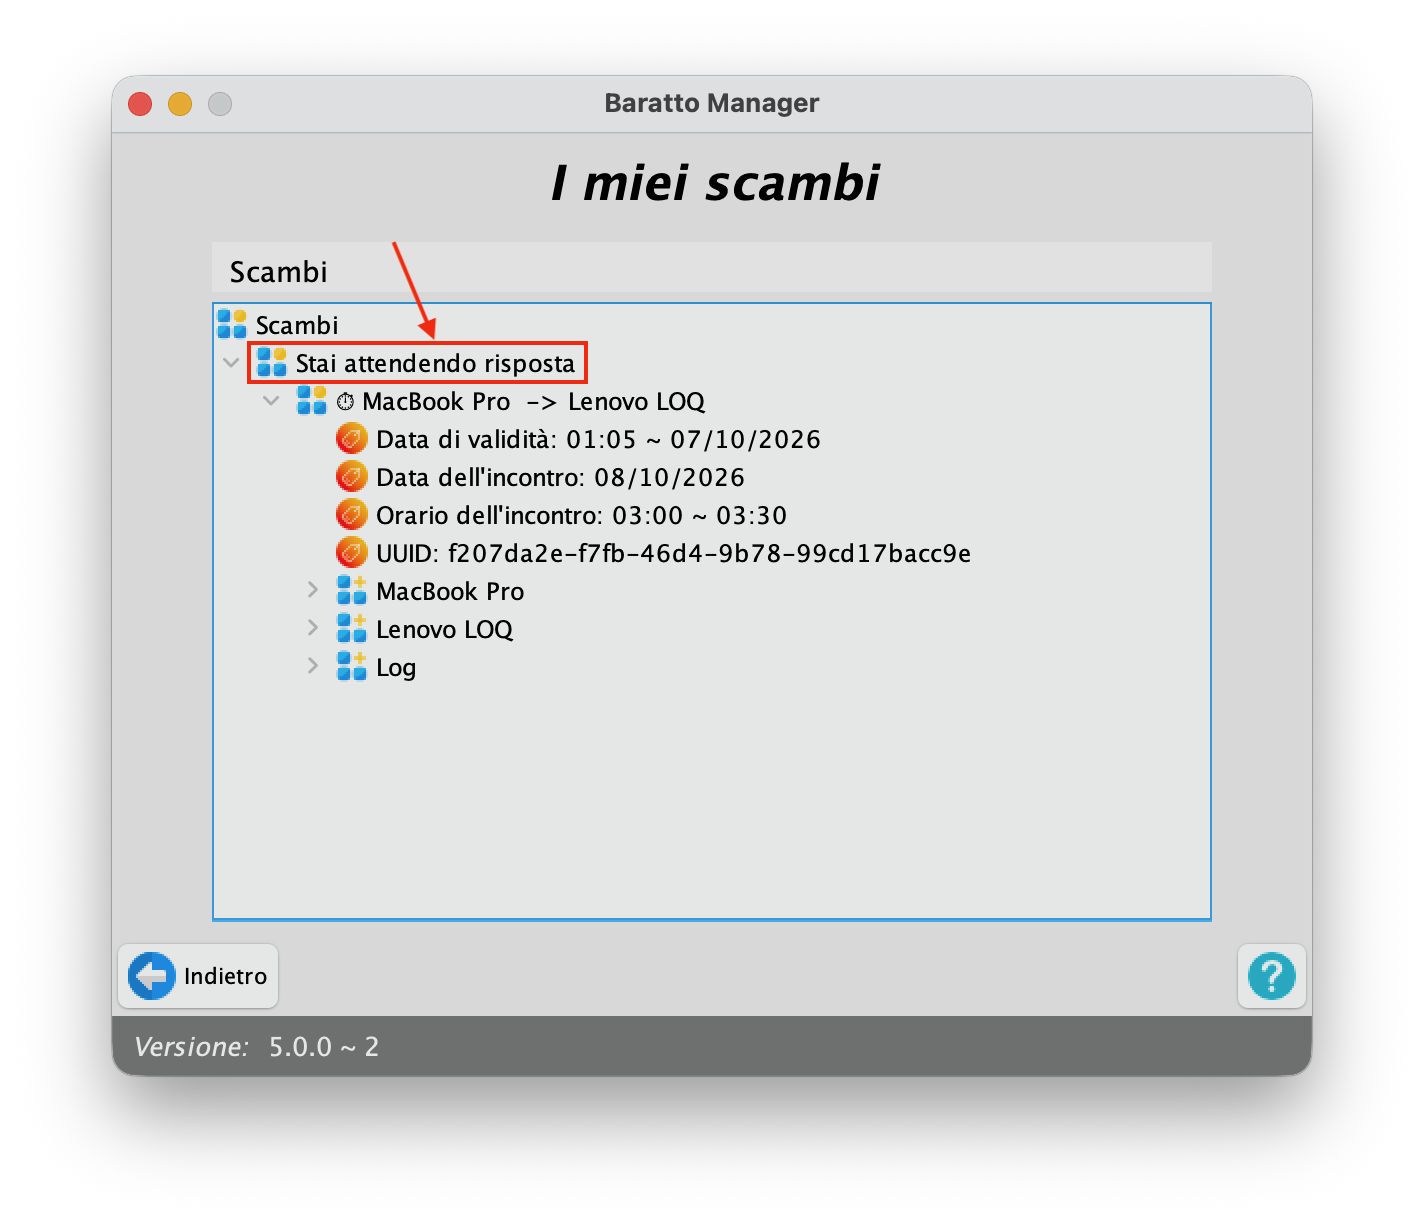
\includegraphics[width=\linewidth]{figures/ss_UI_vecchia/Utente/MieiScambiInAttesa.png}
        \caption{Visualizzazione scambio \textbf{in attesa} di risposta}
    \end{figure}
    \columnbreak
    \begin{figure}[H]
        \centering
        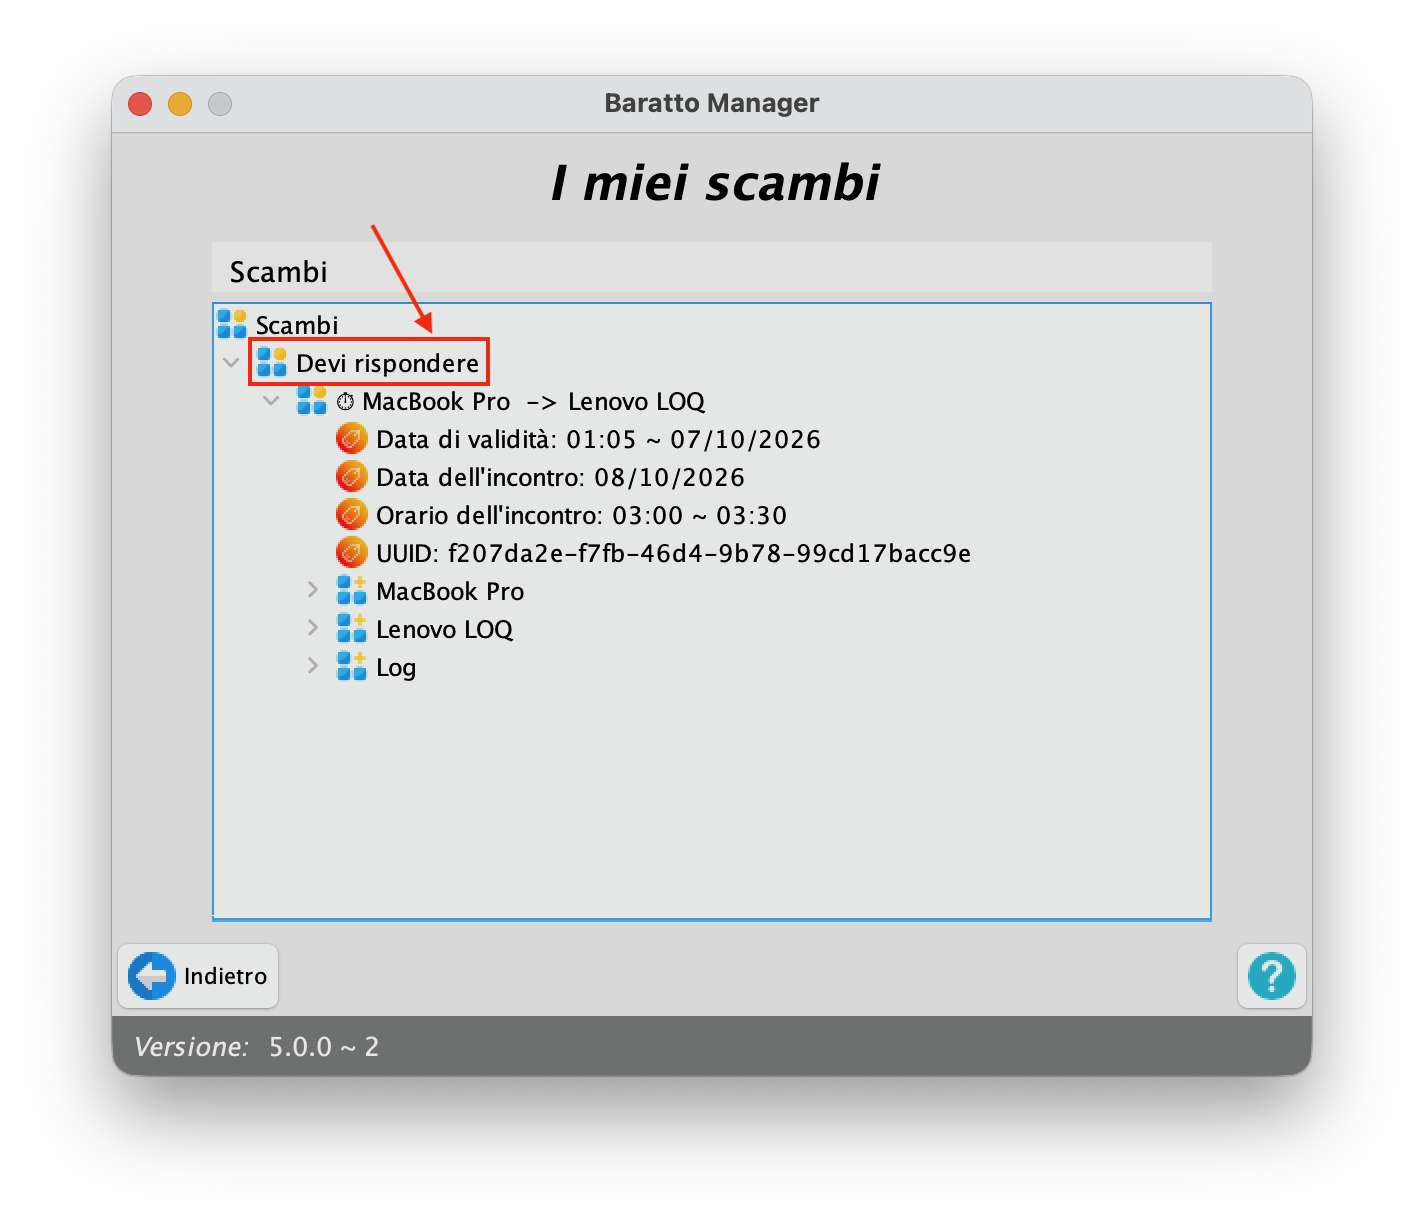
\includegraphics[width=\linewidth]{figures/ss_UI_vecchia/Utente/MieiScambiDaAccettare.png}
        \caption{Visualizzazione scambio \textbf{da accettare}}
    \end{figure}
    \columnbreak
    \begin{figure}[H]
        \centering
        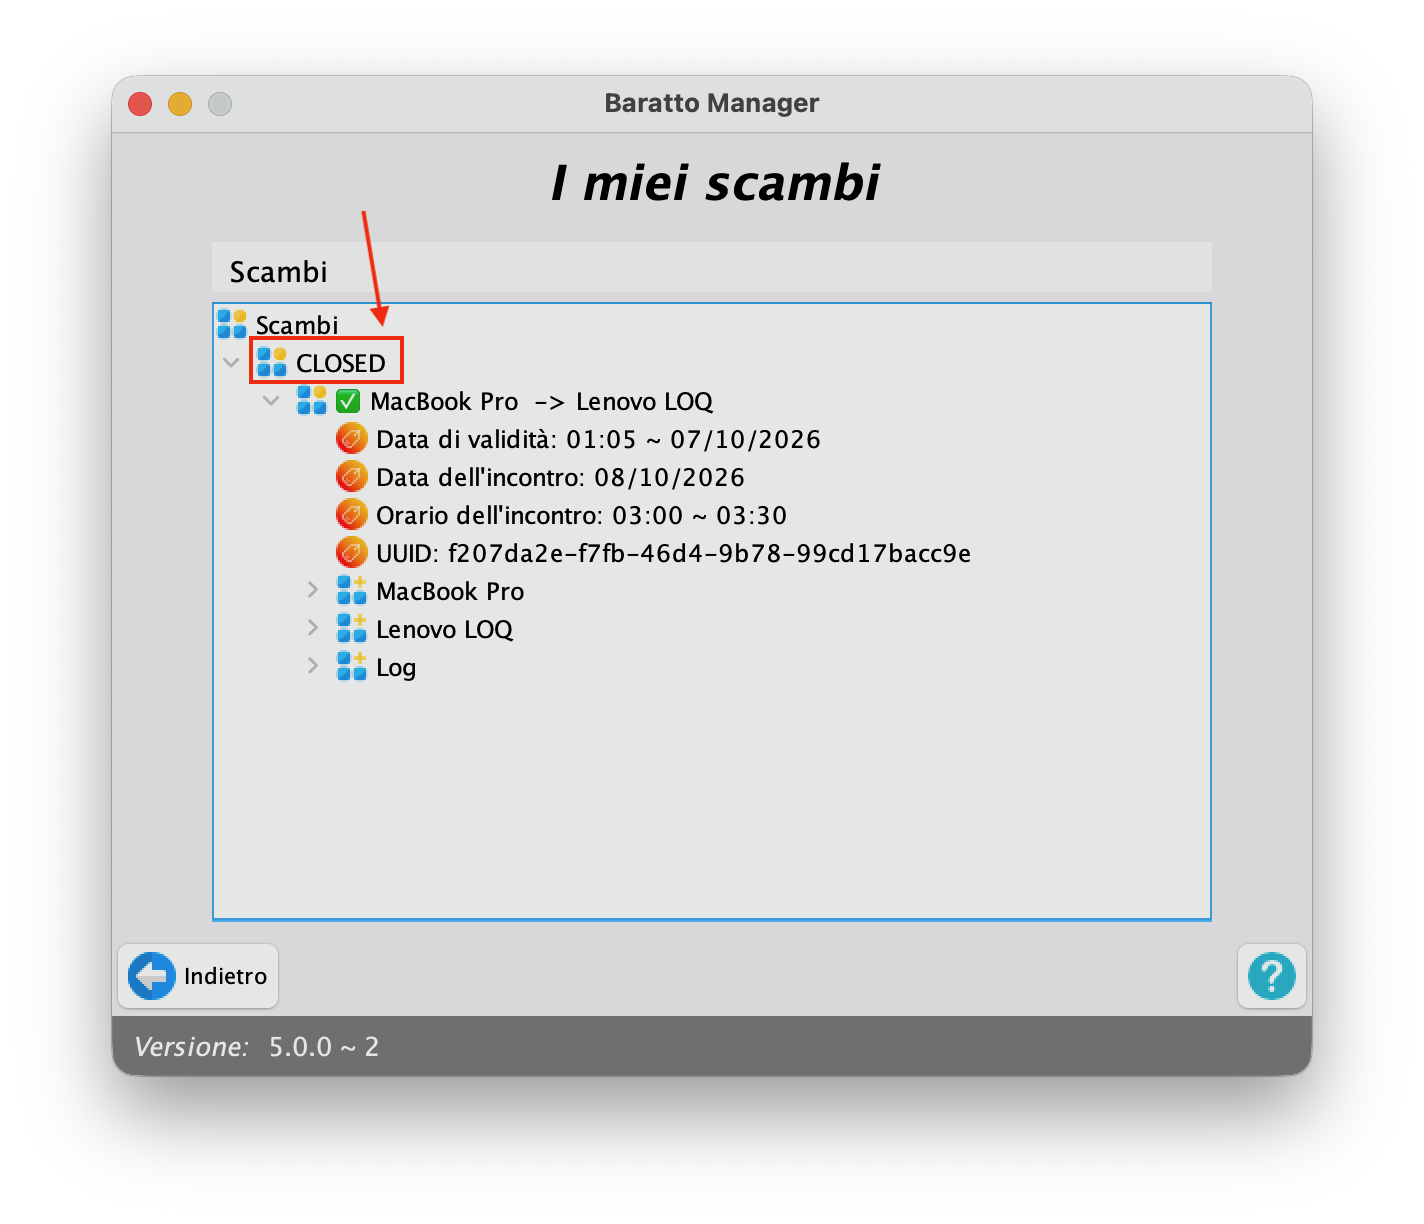
\includegraphics[width=\linewidth]{figures/ss_UI_vecchia/Utente/ScambiClosed.png}
        \caption{Visualizzazione scambio \textbf{chiuso}}
    \end{figure}
\end{multicols*}




\subsection{Pagina di accesso}
La schermata iniziale di accesso è comune a tutti gli utenti.
Si può decidere se accedere o registrarsi.
Nel caso di accesso si inserisce username e password.
Da qui solo gli utenti fruitori hanno la possibilità di registrarsi, indicando uno username. Alla registrazione il sistema assegna una password predefinita, in seguito al primo accesso l'utente viene quindi indirizzato al cambio password, dove deve scegliere una nuova password di almeno 5 caratteri e diversa da quella predefinita.
Dopo l'accesso il sistema mostra la home corrispondente al tipo di utente.

\subsection{Home del configuratore}
Da questa pagina il configuratore può registrare nuovi configuratori, che ricevono anch'essi credenziali predefinite (la registrazione dei configuratori avviene qui e non nella pagina di accesso, per motivi di sicurezza). Può aprire l'editor delle categorie, nel quale aggiunge categorie radice con nome e descrizione, sottocategorie sotto una categoria madre selezionata e campi, indicando per ciascuno se è obbligatorio. Può aggiungere nuovi luoghi di incontro specificando città, via, giorno, orario di inizio e fine e giorni di scadenza per la risposta a uno scambio. Può visualizzare le offerte pubblicate, suddivise per categoria. Infine può caricare un file di configurazione JSON che importa in un'unica operazione categorie, sottocategorie, campi e parametri di configurazione; il sistema rifiuta i file non JSON, quelli con errori di formattazione e i valori già esistenti.

\subsection{Home del fruitore}
Da qui il fruitore può consultare l'elenco delle categorie con relative sottocategorie e campi, e l'elenco dei luoghi di incontro con giorni e orari. Nella sezione "I tuoi articoli" vede i propri articoli con lo stato delle rispettive offerte, può aggiungere un nuovo articolo scegliendo la categoria e compilando i campi richiesti, e può cancellare un'offerta aperta. Nello "Store articoli" vede gli articoli messi a disposizione dagli altri fruitori e può proporre uno scambio: seleziona l'articolo che gli interessa, sceglie un proprio articolo della stessa categoria da offrire in cambio e fissa l'appuntamento tra gli incontri disponibili. Nella sezione "I tuoi scambi" gestisce le proposte ricevute: può accettarle, chiudendo così l'offerta, oppure accettarle proponendo un altro incontro. Se non risponde entro i giorni di scadenza, l'articolo torna allo stato di offerta aperta.
